%%
% BIThesis 本科毕业设计论文模板 —— 使用 XeLaTeX 编译 The BIThesis Template for Undergraduate Thesis
% This file has no copyright assigned and is placed in the Public Domain.
% Compile with: xelatex -> biber -> xelatex -> xelatex
%%

% 请勿删除下面两行注释，以免影响编译。
% !TeX program = xelatex
% !BIB program = biber


% 开启盲审格式 blindPeerReview=true (如：[type=bachelor,blindPeerReview=true])

\documentclass[type=bachelor,blindPeerReview=true]{bithesis}

% 此处仅列出常用的配置。全部配置用法请见「bithesis.pdf」手册。
\BITSetup{
  cover = {
    % 封面需要「北京理工大学」字样图片，如无必要请勿修改该项。
    headerImage = images/header.pdf,
    % 封面标题需要“华文细黑”，如无必要请勿修改该项。
    xiheiFont = STXIHEI.TTF,
    % 可用以下参数自定义封面日期。
    % date = 1955年11月,
  },
  info = {
    % 想要删除某项封面信息，直接删除该项即可。
    % 想要让某项封面信息留空（但是保留下划线），请传入空白符组成的字符串，如"{~}"。
    % 如需要换行，则用 “\\” 符号分割。
    title = 游戏化前端学习移动APP的设计与实现,
    titleEn = {Design and Implementation of a Gamified Front-End Learning Mobile App},
    school = 计算机学院,
    major = 计算机科学与技术（徐特立英才班）,
    class = 07022202,
    author = 雷天慈,
    studentId = 1120223387,
    supervisor = 赵丰年,
    keywords = {游戏化学习；移动学习；前端教育；人工智能辅助；Flutter；学习应用},
    keywordsEn = {gamified learning; mobile learning; front-end education; AI assistance; Flutter; learning application},
    % 如果你的毕设为校外毕设，请将下面这一行语句解除注释（删除第一个百分号字符）并填写你的校外毕设导师名字
    % externalSupervisor = 左偏树,
  },
  style = {
    % 开启 Windows 平台下的中易宋体伪粗体。
    % windowsSimSunFakeBold = true,
    %
    % 开启该选项后，将用 Times New Roman 的开源字体 TeX Gyre Termes 作为正文字体。
    % 这个选项适用于以下情况：
    % 1. 不想在系统中安装 Times New Roman。
    % 2. 在 Linux/macOS 下遇到 `\textsc` 无法正常显示的问题。
    betterTimesNewRoman = true,
  },
  misc = {
    % 微调表格行间距
    tabularRowSeparation = 1.25,
  },
  appendices = {
    chapterLevel = true,
  },
}

% 这份模板提供了代码块示例，采用 listings 宏包及其预定义样式。
% 使用代码块时，也可选用自己的喜欢的其他宏包，如 minted：https://bithesis.bitnp.net/faq/minted.html
% 如果不需要，直接删除即可。
\usepackage{listings}
\usepackage{xcolor}
\lstset{
  basicstyle=\small\ttfamily,
  commentstyle=\color{gray},
  stringstyle=\color{green!50!black},
  numbers=none,
  breaklines=true,
  showstringspaces=false,
  tabsize=2,
  aboveskip=8pt,
  belowskip=8pt,
  backgroundcolor=\color{white},
  frame=none,
}

% Rust language definition for listings
\lstdefinelanguage{Rust}{
  keywords={as, async, await, break, const, continue, crate, dyn, else, enum, extern, false, fn, for, if, impl, in, let, loop, match, mod, move, mut, pub, ref, return, self, Self, static, struct, super, trait, true, type, unsafe, use, where, while, Ok, Err, Some, None, Result, Option},
  keywordstyle=\color{blue}\bfseries,
  ndkeywords={bool, i32, i64, u32, u64, f32, f64, usize, String, Vec, HashMap, PgPool, Request, Depot, StatusError, Json, ApiResponse, Uuid, DateTime, Utc, Value},
  ndkeywordstyle=\color{purple},
  sensitive=true,
  morecomment=[l]{//},
  morecomment=[s]{/*}{*/},
  morestring=[b]",
  morestring=[b]',
  otherkeywords={!,@,#,\$,\%,\&,*,-,+,=,|,<,>,\#,[,],\{,\}},
}

% Dart language definition for listings
\lstdefinelanguage{Dart}{
  keywords={abstract, as, async, await, break, case, catch, class, const, continue, covariant, default, do, dynamic, else, enum, export, extends, extension, external, factory, false, final, finally, for, Function, get, if, implements, import, in, is, late, mixin, new, null, on, operator, part, required, rethrow, return, set, static, super, switch, this, throw, true, try, typedef, var, void, while, with},
  keywordstyle=\color{blue}\bfseries,
  ndkeywords={String, int, double, bool, List, Map, Set, Future, Stream, Widget, BuildContext, GetxController, GetxService, Bindings, Rxn, RxList, RxBool, RxString, RxInt, obs, Obx, GetView, Get},
  ndkeywordstyle=\color{purple},
  sensitive=true,
  morecomment=[l]{//},
  morecomment=[s]{/*}{*/},
  morestring=[b]",
  morestring=[b]',
  otherkeywords={@override,=>,?.},
}

\lstset{language=Rust}

% Custom column type for tables with ragged-right text
\newcolumntype{L}[1]{>{\raggedright\arraybackslash}p{#1}}

% SVG diagrams are pre-converted to PDF via Inkscape, included with \includegraphics

\newcommand{\placeholderfigure}[3]{%
  \begin{figure}[htbp]
    \centering
    \setlength{\fboxsep}{0pt}%
    \fbox{%
      \parbox[c][0.24\textheight][c]{0.82\textwidth}{%
        \centering
        \textbf{图片占位符}\\[0.75em]
        #3
      }%
    }
    \caption{#1}
    \label{#2}
  \end{figure}
}


% 大部分关于参考文献样式的修改，都可以通过此处的选项进行配置。
% 详情请搜索「biblatex-gb7714-2015 文档」进行阅读。
\usepackage[
  backend=biber,
  style=gb7714-2015,
  gbalign=gb7714-2015,
  gbnamefmt=lowercase,
  gbpub=false,
  doi=false,
  url=false,
  eprint=false,
  isbn=false,
]{biblatex}

\makeatletter
\renewbibmacro*{cite:comp:comp}{%
  \cbx@iflabelprefixequalslast
    {\ifnumequal{\thefield{labelnumber}}{\value{cbx@tempcntb}}
       {\savefield{entrykey}{\cbx@lastkey}%
        \savefield{labelnumber}{\cbx@lastnumber}%
        \stepcounter{cbx@tempcnta}}
       {\ifnumequal{\thefield{labelnumber}}{\value{cbx@tempcntb}-1}
          {}
          {\usebibmacro{cite:comp:end}}}}
    {\usebibmacro{cite:comp:end}}%
  % 注释掉下行以禁止编号区间压缩，使引用仅用逗号分隔
  %\setcounter{cbx@tempcntb}{\thefield{labelnumber}}%
  \savefield{labelprefix}{\cbx@lastprefix}}
\makeatother
\addbibresource{misc/ref.bib}

% 减少页面底部过度拉伸，控制每页空白不超过 3 行
\raggedbottom

% 若要按计算机学院要求，添加“北京理工大学”水印，请参考
% https://bithesis.bitnp.net/faq/watermark.html

% 文档开始
\begin{document}

% 标题页面：如无特殊需要，本部分无需改动
\MakeCover

% 原创性声明：盲审结束前无需改动
% 后续添加签名时，可考虑先用 Word 制作再覆盖 misc/1_originality.pdf。
% 不过如无特殊需要，本部分的代码仍无需改动。
\begin{blindPeerReview}
  
\includepdf{misc/1_originality.pdf}\newpage
\end{blindPeerReview}
% \input{misc/1_originality.tex}

% 前置内容定义
\frontmatter
% 摘要：在相应 TeX 文件撰写
%%
% BIThesis 本科毕业设计论文模板 —— 使用 XeLaTeX 编译 The BIThesis Template for Undergraduate Thesis
% This file has no copyright assigned and is placed in the Public Domain.
%%

\begin{abstract}
本文围绕一款面向前端初学者的游戏化学习移动应用的设计与实现展开研究。针对传统前端入门学习中学习动机不足、练习反馈不及时以及移动场景适配不足等问题，论文结合游戏化学习与移动学习的相关理论，设计并实现了一个以移动客户端为核心、服务端与管理后台端为支撑的学习系统。该系统围绕课程学习、章节阅读、编码练习、闯关挑战、每日挑战、社交互动与个人成长反馈等功能构建学习闭环，并通过奖励机制、排行榜和任务节奏增强学习过程的参与感与持续性。

在系统实现上，移动客户端采用 Flutter 进行跨平台开发，结合 GetX 实现路由管理、状态管理与依赖注入，使用 Dio 与 GetStorage 分别完成接口访问与本地持久化；服务端采用 Rust、Salvo 与 PostgreSQL 提供统一业务支撑；同时以 OpenAPI 文档作为三端共享的接口约束基础，用于保证接口结构与联调过程的一致性。论文进一步从需求分析、总体设计、关键功能实现与功能验证四个层面对系统进行说明。

相关实现与验证情况说明，该系统在当前实现范围内能够完成注册登录、课程学习、练习提交、挑战参与、奖励反馈、排行榜展示与基础联调验证等核心流程，能够支撑移动学习闭环的基本运行。本文的工作可为面向前端基础教育场景的移动学习应用设计与实现提供一定参考。
\end{abstract}

\begin{abstractEn}
This thesis studies the design and implementation of a gamified mobile learning application for front-end beginners. To address the problems of weak learning motivation, delayed practice feedback, and insufficient support for mobile learning scenarios in traditional introductory front-end learning, the work combines theories of gamified learning and mobile learning to design and implement a learning system with the mobile application as the core and the server side together with the admin dashboard as supporting components. The system forms a learning loop through course learning, chapter reading, coding practice, level-based challenges, daily challenges, social interaction, and growth feedback, while using rewards, rankings, and task rhythm to strengthen engagement and persistence.

On the implementation side, the learner client is developed with Flutter for cross-platform delivery, uses GetX for routing, state management, and dependency injection, and adopts Dio and GetStorage for API access and local persistence. The server side is implemented with Rust, Salvo, and PostgreSQL to provide unified business support. Meanwhile, an OpenAPI document is used as the shared contract among the mobile client, server side, and admin dashboard to ensure interface consistency during development and integration. The thesis further explains the system from four aspects: requirements analysis, overall design, key function implementation, and functional verification.

The results show that, within the current implementation scope, the system can complete core workflows such as registration and login, course learning, exercise submission, challenge participation, reward feedback, leaderboard display, and basic cross-end integration verification. It therefore demonstrates a relatively complete mobile learning loop and multi-end collaboration capability. The work can provide a useful reference for the design and implementation of mobile learning applications oriented to introductory front-end education.
\end{abstractEn}


\MakeTOC

% 正文开始
\mainmatter

% 在这里引用各章 TeX 文件，按需添加
%%
% BIThesis 本科毕业设计论文模板 —— 使用 XeLaTeX 编译 The BIThesis Template for Undergraduate Thesis
% This file has no copyright assigned and is placed in the Public Domain.
%%

\chapter{绪论}

\section{研究背景}

随着移动互联网终端的普及与碎片化学习方式的发展，基于智能手机开展知识学习已经成为常见的学习场景之一。对于前端基础知识学习而言，HTML 与 CSS 等内容既具有较强的实践性，又要求学习者在理解概念的同时进行持续练习，因此传统以被动阅读为主的学习方式往往难以长期保持学习动机。将积分、徽章、关卡与排行榜等游戏化机制引入学习过程，可增强学习者的参与感与阶段性成就感，同时改善练习反馈的及时性，从而提升学习持续性与主动性。这一方向已有较多研究积累：早期探索可追溯至基于计算机的教育游戏实践\cite{cullingford1979}，之后 Prensky 正式提出数字游戏化学习概念\cite{prensky2000}，并从视频游戏与学习的关系出发积累了理论基础\cite{squire2003,gee2003}；Hwang 等人\cite{hwang2012}、Dicheva 等人\cite{dicheva2015} 及 Qian 和 Clark\cite{qian2016} 的综述工作进一步梳理了数字游戏化学习的研究脉络，Clark 等人\cite{clark2016} 的元分析验证了游戏化设计对学习效果的促进作用；在移动学习方面，Godwin-Jones\cite{godwinjones2011} 对移动应用在语言学习中的应用进行了分析，Sung 和 Hwang\cite{sung2018}、Li 和 Tsai\cite{li2013} 分别从协作建构和科学教育视角探讨了游戏化学习的移动化趋势\cite{deterding2011,hamari2014,ryan2000}。

移动学习强调学习过程与时间、地点的解耦，使学习者能够在通勤、课余等碎片时间中完成短时高频的学习活动。对于前端入门教育而言，若能够结合课程阅读、编码练习、闯关挑战、每日任务与社交反馈等机制，构建面向移动客户端的完整学习闭环，则有助于提升学习过程的连贯性和趣味性，并为前端基础能力培养提供更具交互性的支持环境\cite{liang2018,jiao2023}。

前端技术作为 Web 开发的基础，其学习需求持续增长。HTML 负责页面结构，CSS 负责页面样式，两者共同构成了 Web 页面的基础。对于初学者而言，这些技术虽然入门门槛相对较低，但要达到熟练运用水平仍需要大量实践。传统的学习方式主要依赖教材阅读和静态示例观摩，学习者难以获得及时的练习反馈和进度确认。游戏化学习应用则通过将学习内容组织为任务链、将练习过程设计为挑战关卡、将学习成果可视化为成长数据，在一定程度上弥补了传统方式的不足，为前端基础教育提供了更具吸引力的学习载体。

\section{研究目的与意义}

本文面向前端初学者，围绕一款游戏化前端学习移动应用的设计与实现展开研究，目标是构建一个以移动客户端为核心的学习系统，使学习者能够在课程学习、代码练习、挑战通关、每日任务与社交激励的协同作用下完成前端基础知识的持续学习。系统在功能上强调学习闭环的完整性，在实现上强调移动客户端体验与服务端、管理后台端协同的一致性。

在实践层面，该系统尝试将游戏化学习机制与移动学习场景结合，探索更适合前端基础教育的应用实现方式。游戏化机制在教育领域的应用已有较多研究，但面向前端技术学习、以移动应用为载体的系统化实现案例仍然较少。本系统通过将课程学习、编码练习、挑战机制和社交反馈整合到移动客户端中，为前端初学者提供了一种新的学习途径，其实践价值在于验证这种整合方式的可行性，并为后续效果评估提供实现基础。

工程层面，本文通过移动客户端、服务端、管理后台端与契约文档之间的协同设计，形成一套可落地的多端联动实现方案，为同类学习应用的设计与开发提供参考\cite{sommerville2015,sylvester2013,kalmpourtzis2018}。系统涉及移动应用开发、服务端构建、管理界面开发和接口契约维护等多个技术领域，这些领域之间的协同工作是系统成功落地的关键。本文在实现过程中积累的多端协作经验和技术选型思考，对于其他需要类似架构的学习应用具有一定的参考价值。

\section{国内外研究现状}

现有研究表明，游戏化通过在非游戏环境中引入游戏设计元素，可以对学习动机、学习投入与持续使用行为产生积极影响，但其具体效果仍与学习情境、任务设计与用户特征密切相关。教育游戏、游戏化学习与移动学习在目标、方法与应用侧重点上存在差异，研究者通常需要结合具体学习对象与学习目标进行设计，而不能简单依赖单一游戏元素获得稳定效果。Hamari 等人\cite{hamari2016} 对挑战性游戏在学习中的作用进行了实证研究，发现适当的挑战水平与心流体验、沉浸感存在密切联系；Woo\cite{woo2014} 和 Zyda\cite{zyda2005} 分别从学习动机与仿真技术演进角度讨论了数字游戏应用于教育的可行路径\cite{deterding2011,hamari2014,kalmpourtzis2018}。

Deterding 等人对游戏化的定义和构成要素进行了系统梳理，为后续研究提供了概念基础。Hamari 等人通过文献综述发现，游戏化在教育领域的应用效果存在较大差异，其成功依赖于游戏元素与学习目标的匹配程度。Kalmpourtzis 从教育游戏设计角度指出，有效的游戏化设计需要深入理解学习者的动机结构和认知特征，而非简单套用游戏机制。这些研究为本系统的设计提供了理论指导，使游戏化机制的选择更加注重与学习内容的契合度。

人工智能教育领域也出现了重要进展。Luckin 和 Holmes\cite{luckin2016} 系统地论述了人工智能在教育中的应用前景，指出 AI 可在个性化辅导、智能评测和学习路径推荐等方面发挥关键作用；LeCun 等人\cite{lecun2015} 对深度学习技术的系统阐述为智能教育工具提供了核心算法支撑，使基于神经网络的自动评测和错误分析成为可能；Jia 等人\cite{jia2024} 对近十年 AI 在科学教育中的研究趋势进行了系统回顾，发现 AI 教育研究正从工具开发向学习效果验证转变；Kandlhofer 等人\cite{kandlhofer2021} 从机器人教育标准化角度提出了系统的培训框架；Renz 和 Hilbig\cite{renz2020} 则从技术采纳角度分析了 AI 在教育领域的驱动因素和障碍。同时，Drigas 和 Ioannidou\cite{drigas2013} 以及 Xie 等人\cite{xie2019} 的研究分别从特殊教育与自适应学习角度丰富了技术增强学习的研究图谱，前者展示了 ICT 技术如何为特殊需求学习者提供差异化支持，后者通过系统综述揭示了自适应学习系统从规则驱动向数据驱动演进的趋势\cite{koedinger1997,woolf2010,brusilovsky2007,papamitsiou2014}。

智能辅导系统研究关注如何通过计算机程序模拟人类教师的一对一辅导过程，为学习者提供个性化的学习指导。Koedinger 等人的研究表明，智能辅导系统能够有效提升学习效果，但其开发成本和技术复杂度较高。自适应教育系统研究则关注如何根据学习者的实时表现动态调整学习内容和路径，Brusilovsky 等人对用户建模和自适应策略进行了系统总结。学习分析技术研究关注如何从学习行为数据中提取有价值的信息，Papamitsiou 等人的综述显示了该领域从理论探索向实践应用的转变趋势。本系统虽然未实现完整的智能辅导或自适应推荐功能，但在进度记录、错误提示和成就反馈等方面借鉴了这些研究的思路。

编程教育与 Web 开发教学领域的研究重点主要集中在编程入门难点、教学支撑工具、Web 开发学习方式以及程序可视化辅助等方面。编程学习既依赖知识讲解，也依赖可操作、可反馈、可重复的实践过程，这与游戏化学习应用强调任务驱动和即时反馈的设计逻辑具有一定一致性\cite{robins2003,heines2001,guo2013}。

Robins 等人对编程教学中的困难进行了系统分析，指出概念理解、错误定位和知识迁移是初学者面临的主要挑战。Heines 的研究表明，Web 开发教学需要特别关注实践环节的设计，使学习者能够在接近真实的环境中进行练习。Guo 开发的 Python Tutor 工具展示了程序可视化在编程教育中的价值，通过图形化展示程序执行过程帮助学习者理解代码行为。这些研究为本系统的练习设计和反馈机制提供了参考，使编码练习环节更加注重错误提示的可理解性和学习过程的可视化。

从现有产品的对比分析来看，市场上已经出现了一批面向编程教育的移动学习应用，例如 Sololearn、Mimo 和 Programming Hero 等。Sololearn 以社区驱动的内容和短小精悍的课程单元为特色，但其游戏化机制主要体现为基础积分和经验值积累，缺乏对编码练习结果的深度反馈和挑战式任务组织；Mimo 在移动客户端交互设计上较为精致，但其内容更偏向通用编程入门，对 HTML/CSS 前端方向的专项覆盖有限；Programming Hero 将 RPG 叙事与编程练习结合，游戏化体验较强，但其服务端架构和接口契约细节未公开，难以作为多端协同工程的参考案例。这些产品的共同不足在于：或缺乏前端专项内容体系，或未深度整合游戏化机制与编码练习反馈链路，或未提供多端协同架构的工程参考。本文正是在这一差异化空间上展开工作，尝试将游戏化学习机制、前端基础知识体系和契约优先的多端工程方法进行整合。

综上，现有研究为游戏化学习、智能教育支持与编程教学提供了理论基础，但面向前端基础教育场景、以移动应用为主体、结合课程学习、代码练习、挑战机制与社交反馈的系统化实现案例仍具有较强的实践研究价值。

\section{研究内容与论文结构}

本文以游戏化前端学习移动应用为研究对象，对系统的需求分析、总体设计、关键功能实现与功能验证过程进行梳理和总结。论文内容主要包括相关理论与关键技术、系统需求分析、系统设计、系统实现与测试等部分。其中，移动客户端学习应用为全文叙事主体，服务端与管理后台端作为支撑系统，OpenAPI 工具链作为协同约束手段，共同用于保证学习流程闭环与系统协同实现。

全文共分为五章。第一章为绪论，介绍研究背景、研究意义、研究现状与论文结构；第二章为相关理论与关键技术，说明游戏化学习、移动学习及系统开发所涉及的关键技术；第三章为需求分析，梳理系统的总体需求、功能需求与非功能需求；第四章为系统设计，说明系统总体架构、功能结构、业务流程与接口协同方式；第五章为系统实现与测试，介绍开发环境搭建、开发过程、移动客户端与服务端管理后台端关键实现，以及系统功能验证与联调情况。

在叙事逻辑上，本文始终围绕移动客户端学习体验展开，服务端和管理后台端作为支撑系统配合说明。这种组织方式既保证了论文焦点的集中，又体现了系统实现的多端协同特征。各章节之间保持逻辑递进关系，从理论基础到需求分析，从系统设计到实现测试，逐步展开。

本文的研究范围限定在系统的设计与实现层面。系统通过学习进度记录、经验值变动、提交历史和连续学习天数等数据，记录了学习者的学习行为轨迹，这些数据可为后续的教学效果实验和用户行为分析提供数据基础，但本文不涉及对这些数据的教学效果评估或用户行为统计建模。这种范围界定既符合本科毕业设计的实际条件，也使论文能够聚焦于工程实现层面的深入分析。

方法论上，本文采用工程实践与文献分析相结合的方式推进。工程实践方面，通过实际的系统开发过程验证设计方案的可行性，在开发过程中不断调整和完善设计决策。文献分析方面，通过查阅游戏化学习、移动教育和编程教学等领域的相关研究，为系统设计提供理论支撑。这种理论与实践相互支撑的方法使系统既有理论依据，又具备实际可行性。

在创新贡献方面，本文的价值不在于提出全新的游戏化理论或突破性的技术方案，而在于将已有的游戏化学习理念与前端基础教育场景相结合，通过移动客户端、服务端和管理后台端的协同实现，构建了一个可运行的学习应用原型。其意义在于探索了游戏化机制在前端技术学习领域的具体应用方式，以及多端协同架构在移动学习场景中的实现路径，为后续研究和实践提供了参考案例和基础平台。

前端技术学习具有知识更新快、实践性强和学习者基数大的特点。传统的课堂教学和在线教程虽然能够覆盖知识传授环节，但在学习动机维持、实践反馈及时性和学习进度可视化等方面存在不足。本系统尝试通过移动客户端将学习过程游戏化，使学习者能够在碎片化时间中完成短时高频的学习活动，并通过积分、徽章、排行榜等机制获得即时的正向反馈。这一设计思路对于其他需要大量实践练习的技术学习领域——如后端开发、移动应用开发和数据科学等方向的基础教育——也具有一定的借鉴意义。

%%
% BIThesis 本科毕业设计论文模板 —— 使用 XeLaTeX 编译 The BIThesis Template for Undergraduate Thesis
% This file has no copyright assigned and is placed in the Public Domain.
%%

\chapter{相关理论与关键技术}

\section{游戏化学习相关理论}

游戏化学习强调在非游戏情境中引入积分、徽章、等级、任务、反馈与排行榜等游戏设计元素，以提高学习活动的参与度和持续性。与完整的教育游戏相比，游戏化更关注将游戏机制嵌入既有学习任务之中，使学习者在完成真实学习目标的过程中获得更强的行为激励与过程反馈。对于前端基础知识学习而言，课程阅读、代码练习与阶段性挑战天然具有任务化特征，因此较适合与游戏化机制进行结合\cite{deterding2011,hamari2014,sylvester2013}。

从学习动机角度看，游戏化机制能够通过即时反馈、阶段奖励和目标可视化增强学习者的胜任感与进度感。当学习者完成一道练习或通过一个关卡时，系统立即给予积分、徽章或等级提升等反馈，这种即时正向强化有助于建立学习与奖励之间的关联，增强学习行为的持续性。对初学者而言，这种设计有助于缓解前端入门阶段中因知识抽象、练习反复与错误频发所带来的挫败感，提高其继续学习的意愿。因此，在本系统中，积分奖励、关卡挑战、每日任务和排行榜并不是附加装饰，而是服务于学习行为持续发生的交互机制。这一思路与自我决定理论中关于自主性、胜任感和归属感的解释相一致\cite{ryan2000,kalmpourtzis2018}。

自我决定理论认为，人类有三种基本心理需求：自主性需求、胜任感需求和归属感需求。在游戏化学习环境中，自主性需求体现为学习者可以选择学习路径、挑战难度和学习节奏；胜任感需求体现为通过任务完成和技能提升获得的能力确认；归属感需求体现为通过排行榜、好友互动等社交机制获得的群体认同。本系统在设计时考虑了这三种需求的平衡，既提供结构化的课程路径保证学习系统性，又通过挑战选择和社交功能给予学习者一定的自主空间。

\section{移动学习与智能教育支持}

移动学习强调学习者能够借助移动终端在不同时间、不同地点完成学习活动，其核心特征包括学习场景灵活、学习过程碎片化、交互方式轻量化以及设备依赖性明显。与桌面环境相比，移动客户端在屏幕空间、输入方式、网络稳定性与操作节奏方面存在天然限制，因此移动学习应用在设计时需要更加重视信息层级、任务流程、反馈节奏与离线容错能力\cite{liang2018,jiao2023}。

移动学习的碎片化特征意味着学习者通常只能在较短时间内集中注意力，单次学习时长可能只有几分钟到十几分钟。这种特征对学习内容的设计提出了特殊要求：内容单元应足够紧凑，使学习者能够在一次碎片时间内完成一个完整的学习任务；进度保存应足够及时，使学习者可以随时中断并在下次继续；反馈应足够迅速，使学习者能够在有限时间内获得学习效果的确认。本系统的章节设计、练习长度和每日挑战难度都考虑了这种碎片化特征，力求使每个学习单元都能在典型碎片时间内完成。

在教育技术发展过程中，智能辅导系统、自适应教育系统与学习分析方法不断丰富，为学习资源推荐、学习路径调整、学习行为记录与反馈设计提供了重要参考。虽然本文并不以构建复杂智能教学系统为核心目标，但这些研究为系统中的辅助提示、进度记录和成长反馈设计提供了理论借鉴\cite{koedinger1997,woolf2010,brusilovsky2007,papamitsiou2014}。

智能辅导系统的核心思想是通过建模学习者的知识状态，提供个性化的教学指导和练习推荐。自适应教育系统则进一步关注学习路径的动态调整，根据学习者的表现实时改变后续内容的难度和类型。学习分析技术通过收集和处理学习行为数据，为教学决策和系统优化提供数据支持。本系统虽然未实现完整的知识追踪模型或自适应推荐算法，但在进度记录、错误提示和成就反馈等方面借鉴了这些研究的思路，为后续功能扩展预留了空间。

\section{前端学习与编程教学相关支撑}

前端基础学习兼具知识理解与实践操作双重特征，因此其教学过程既需要结构化内容呈现，也需要可反馈的编码练习环境。编程教育研究普遍认为，程序设计教学中的困难主要体现在抽象概念理解、错误定位、实践反馈以及学习迁移等方面。初学者在学习 HTML 和 CSS 时，常常难以理解抽象的标签语义和样式规则，更难将所学知识应用到新的页面布局场景中。与此相应，Web 开发教学与程序可视化工具研究说明，良好的交互反馈和过程可视化能够降低学习门槛，提高学习者的理解效率和练习积极性\cite{robins2003,heines2001,guo2013}。

在错误定位方面，前端代码的错误往往不会导致程序崩溃，而是表现为页面显示异常，这种静默失败特征增加了初学者定位问题的难度。因此，系统在设计练习反馈时，不仅返回测试用例是否通过的结果，还尽可能提供具体的错误描述和修正建议，帮助学习者理解问题所在。在学习迁移方面，系统通过不同难度的挑战任务和多样化的练习场景，促使学习者将基础知识应用到不同的实际问题中，逐步培养灵活运用能力。

本系统以 HTML 与 CSS 为前端学习切入点，通过课程内容、代码练习、挑战关卡和成长反馈相结合的方式组织学习流程，其设计思路与上述研究在实践训练和即时反馈方面具有一致性。HTML 作为页面结构描述语言，其学习重点在于理解各种标签的语义和适用场景；CSS 作为页面样式描述语言，其学习重点在于理解选择器、盒模型、布局方式等核心概念。这两部分内容既相互独立又紧密关联，系统通过课程组织使学习者先分别掌握基础知识，再通过综合练习和挑战将两者结合运用。

\section{系统实现相关技术}

从工程实现角度看，学习应用的构建不仅依赖教育理论，也依赖稳定的软件工程方法和适合的技术实现路径。软件工程理论为需求梳理、系统分层、模块协作与后续维护提供了方法基础，而游戏设计与教育游戏设计相关研究则为任务组织、反馈节奏和学习体验构建提供了实践参考\cite{sommerville2015,sylvester2013,kalmpourtzis2018,campos2022}。

软件工程方法强调通过需求分析、系统设计、实现和测试等阶段有序推进项目，在每个阶段建立明确的交付物和验证标准。本系统的开发过程遵循这一基本流程，在需求分析阶段明确功能范围和非功能约束，在系统设计阶段确定架构方案和技术选型，在实现阶段按模块逐步开发，在测试阶段验证功能正确性和接口一致性。这种分阶段推进方式有助于控制项目风险，使问题能够在早期被发现和解决。

本文在技术实现上采用移动客户端、服务端与管理后台端协同的方式完成系统搭建。移动客户端选择 Flutter 框架进行跨平台开发，使同一套代码能够同时构建 iOS 和 Android 应用，降低多端维护成本。服务端选择 Rust 语言和 Salvo 框架，利用 Rust 的内存安全特性和高性能特征，为移动客户端提供稳定可靠的接口服务。管理后台端选择 Vue.js 框架，借助其组件化开发模式和丰富的生态，快速构建运营人员使用的管理界面。

相关技术选择服务于系统工程落地，而非作为论文创新点单独展开。其核心价值在于支撑课程学习、编码练习、挑战反馈与多端联动的整体实现。在技术选型时，优先考虑了团队熟悉度、社区活跃度和文档完善度等因素，使技术风险控制在可接受范围内。同时，技术栈的确定也考虑了后续维护和功能扩展的需求，选择了具有良好生态和持续发展潜力的技术方案。

Flutter 框架采用 Dart 语言开发，通过自绘渲染引擎实现跨平台一致性，其热重载特性能够显著提升开发迭代效率。在移动客户端开发中，Flutter 的 Widget 系统提供了丰富的界面构建能力，使开发者能够以声明式方式描述界面结构和交互行为。GetX 作为 Flutter 的状态管理方案，提供了依赖注入、路由管理和状态响应式更新等能力，其轻量级特性适合中小型项目的快速开发。

Rust 语言以其内存安全保证和零成本抽象著称，适合构建需要高可靠性的服务端应用。Salvo 作为 Rust 生态中的 Web 框架，提供了异步请求处理、中间件支持和路由组织等基础能力，其设计理念与 Rust 语言特性相契合，能够在保证性能的同时提供较好的开发体验。在服务端开发中，异步编程模型能够有效处理并发请求，而 Rust 的所有权系统则在编译期避免了常见的内存安全问题。

Vue.js 作为渐进式前端框架，其组件化开发模式和响应式数据绑定机制使界面开发更加高效。在管理后台端开发中，Vue.js 的单文件组件结构使模板、脚本和样式能够集中管理，配合 Element Plus 等组件库可以快速构建功能完善的管理界面。Axios 作为 HTTP 客户端库，提供了请求拦截、响应处理和错误管理等能力，与服务端接口的对接过程较为顺畅。

在接口契约方面，系统采用 OpenAPI 规范描述接口定义，使三端能够在统一的文档基础上进行开发和联调。OpenAPI 文档作为三端共享契约，并可用于导出接口文档页面，提高开发沟通的一致性。在数据持久化方面，系统采用关系型数据库存储业务数据，通过合理的表结构设计和索引优化保证基础查询性能。在数据迁移方面，系统使用迁移脚本管理数据库模式变更，使开发和生产环境的数据库结构能够保持一致，便于团队协作和版本控制。

综合来看，本系统的技术选型遵循了实用性、可维护性和可扩展性原则，各技术组件之间形成了较为合理的分工协作关系。移动客户端负责用户交互和状态管理，服务端负责业务逻辑和数据处理，管理后台端负责内容运营和系统配置，接口契约负责多端协同的标准化。这种技术架构既满足了当前功能需求，也为后续功能扩展和性能优化预留了空间。

%%
% BIThesis 本科毕业设计论文模板 —— 使用 XeLaTeX 编译 The BIThesis Template for Undergraduate Thesis
% This file has no copyright assigned and is placed in the Public Domain.
%%

\chapter{需求分析}

\section{总体需求分析}

本系统面向前端初学者构建移动客户端学习环境，目标是在移动设备上形成课程学习、代码练习、闯关挑战、每日任务、社交激励与个人成长相结合的完整学习闭环。根据需求文档，系统由移动客户端、服务端与管理后台端组成，其中移动客户端承担主要学习活动，服务端负责统一业务处理与数据支撑，管理后台端负责内容维护、运营支撑与数据管理。该类系统既需要满足移动学习场景下的便捷访问需求，也需要兼顾编程教育中实践反馈及时、任务组织明确和学习持续性较强等特点\cite{robins2003,heines2001,sommerville2015}。

从学习目标上看，系统不仅要支持前端基础知识的呈现和阅读，还应支持学习者通过编码练习和挑战任务完成知识内化，并借助成长反馈与社交激励增强持续学习意愿。因此，系统需求不能只停留在内容展示层面，而需要覆盖学习行为记录、任务组织、结果反馈和成长激励等多个方面\cite{hamari2014,ryan2000,kalmpourtzis2018}。前端基础知识包括 HTML 标记语言、CSS 样式语言和基础页面布局等内容，这些知识既具有明确的语法规则，又需要通过大量实践才能熟练掌握，因此系统需求特别强调理论与实践的结合。

从用户群体特征来看，目标用户主要是前端初学者，他们可能具备一定的计算机使用经验，但对 Web 开发技术尚不熟悉。这类用户在学习过程中容易因概念抽象、错误难以定位或缺乏及时反馈而产生挫败感，因此系统需要在交互设计上注重引导性、反馈的及时性和错误提示的可理解性。同时，初学者通常没有固定的学习时间和场所，移动学习场景正好契合其利用碎片时间学习的需求，但也对系统的离线能力和状态恢复能力提出了更高要求。

从系统边界来看，本文聚焦于学习应用本身的设计与实现，不包括完整的在线代码执行环境、大规模用户行为分析系统或商业化运营平台。AI 辅助功能限定在错误解释和提示层面，不扩展为完整的智能辅导系统。社交功能限定在好友、动态和排行榜等基础互动形式，不扩展为实时通信或协作编程等复杂场景。这些边界界定使系统需求保持在一个可实现的范围内，同时为核心学习闭环的完整性提供保障。

\section{技术需求分析}

在运行平台方面，移动客户端需要支持 iOS 与 Android 智能手机，适配不同尺寸屏幕并保持基础交互一致性；管理后台端主要面向桌面浏览器环境，用于内容维护与配置操作；服务端需要具备面向多端的统一 API 提供能力。由于系统存在移动客户端学习场景，因此网络环境不能假设始终稳定，应用需要具备一定的离线感知与本地缓存能力\cite{liang2018,jiao2023}。

移动客户端的技术需求还包括对移动设备特性的适配。例如，需要处理不同屏幕尺寸和分辨率的布局适配问题，需要在虚拟键盘弹出时调整界面元素位置，需要处理应用前后台切换时的状态保存和恢复。在性能方面，移动客户端需要控制内存占用和电量消耗，避免长时间使用导致设备过热或电量快速下降。在存储方面，移动客户端需要合理利用本地存储空间，对缓存数据进行有效管理，避免因存储膨胀影响应用性能。

在系统协同方面，服务端接口必须能够同时支撑移动客户端与管理后台端的访问需求，并通过统一响应结构保障调用一致性。与此同时，接口文档需要作为开发与联调的共同依据，以减少多端协作中的理解偏差。对移动客户端而言，还需要具备认证信息持久化、进度缓存、弱网回退与错误处理能力，以保证学习流程的连续性\cite{brusilovsky2007,papamitsiou2014,sommerville2015}。

服务端的技术需求还包括对并发访问的处理能力、对数据库操作的事务保障、对异常情况的容错处理等。虽然本文不涉及大规模性能优化，但服务端需要保证在正常负载下能够稳定响应请求，在异常情况下能够给出合理的错误信息而不是直接崩溃。管理后台端的技术需求则侧重于内容编辑的便利性、数据展示的清晰性和操作反馈的及时性，使运营人员能够高效地完成日常维护工作。

\section{功能需求分析}

结合需求文档与现有实现，移动客户端功能可归纳为以下几个方面。第一是账户管理功能，包括注册、登录与个人资料维护，用于建立用户身份与学习档案。第二是课程学习功能，包括课程列表浏览、课程详情查看、章节阅读和学习进度跟踪，用于支撑基础知识学习过程。第三是编码练习功能，包括练习详情查看、代码提交与结果反馈，用于连接知识理解与实践操作\cite{robins2003,heines2001,guo2013}。

第四是挑战相关功能，包括闯关挑战、星级评价、奖励发放与每日挑战，用于将学习活动组织为具有目标感与节奏感的任务链。第五是 AI 辅助功能，用于在学习者练习受阻时提供错误解释与必要提示，但其范围应限定在辅助解释层面，而不扩展为完整的代码生成或个性化推荐系统。第六是社交互动功能，包括好友、动态与排行榜，用于提供外部激励与学习氛围。第七是成长反馈功能，包括经验值、徽章、等级与统计信息，用于沉淀学习成果并强化用户成长感知\cite{koedinger1997,woolf2010,liang2018,jiao2023}。

在账户管理功能中，注册流程需要收集用户基础信息并验证输入有效性，登录流程需要验证身份并发放认证凭证，个人资料维护需要支持昵称、头像等信息的修改。这些功能虽然基础，但直接影响用户首次使用体验和后续身份识别，因此需要在易用性和安全性之间取得平衡。

在课程学习功能中，课程列表需要支持分类筛选和搜索，课程详情需要展示完整的课程信息和章节目录，章节阅读需要提供舒适的内容展示和进度记录。学习进度跟踪需要记录每门课程、每个章节的学习状态，使学习者能够随时了解自己的学习进展，也为系统的个性化推荐和成长反馈提供数据基础。

在编码练习功能中，题目展示需要清晰说明要求和示例，代码编辑需要提供基础的输入环境，结果反馈需要及时返回编译和测试结果。这些功能的实现质量直接影响学习者的练习体验，特别是错误反馈的可理解性，对于帮助初学者定位和修正错误至关重要。

对于支撑系统而言，管理后台端需具备课程、题目、挑战、用户与公告等内容管理能力，以支持移动客户端的内容供给与日常运营；服务端则需提供统一的认证、内容访问、提交记录、奖励结算、进度管理与社交数据接口，从而保证学习闭环能够在多端环境中稳定运行\cite{sommerville2015,campos2022}。

\section{非功能需求分析}

在可用性方面，系统应保证学习者能够以较短路径完成主要学习任务，界面反馈应清晰，状态切换应明确，减少因复杂操作造成的学习中断。具体而言，从打开应用到进入课程学习的操作步骤应控制在三步以内，常用功能应在主界面直接可达，避免深层嵌套的导航结构。错误提示应使用学习者能够理解的语言，避免展示技术性错误代码或堆栈信息\cite{heines2001,guo2013}。

在响应性方面，系统需要保证课程加载、页面切换、请求返回与错误反馈具备基本可接受的交互速度，并能在网络异常时给出可理解的提示。课程列表和章节内容的加载时间应控制在用户可接受的范围内，代码提交后的结果反馈应尽可能及时，避免学习者因等待时间过长而产生焦虑。在网络异常时，系统应明确告知用户当前网络状态，并提供重试或稍后操作的选项，而不是无限等待或显示空白页面。

在可维护性方面，移动客户端、服务端与管理后台端应保持职责清晰，接口结构统一，便于后续功能扩展与问题定位。代码组织应遵循模块化原则，各功能模块之间的耦合度应控制在合理范围内，使单个模块的修改不会对其他模块产生意外影响。文档应覆盖关键设计决策和接口定义，使新加入的开发者能够快速理解系统结构。

在一致性方面，系统需要通过统一契约文档控制接口字段、响应包络与权限边界，保证多端协作不因接口漂移而失效。移动客户端的界面风格应保持一致，相同功能的交互方式应在不同页面中遵循相同模式，减少学习者的认知负担。服务端对同类请求的处理逻辑应保持一致，避免因特殊处理导致的意外行为。

在可靠性方面，移动客户端应支持本地存储和离线回退策略，使学习记录不会因为短时断网而直接丢失。关键操作如代码提交应在本地保存副本，网络恢复后自动重试提交，避免因网络抖动导致学习成果丢失。服务端应保证数据持久化的可靠性，对关键操作采用事务保障，避免部分更新导致的数据不一致。

在扩展性方面，系统需要为后续课程扩充、挑战增加和能力增强保留一定结构空间，但本文只围绕当前实现范围展开，不对后续版本功能进行详细设计\cite{sommerville2015,papamitsiou2014}。具体而言，课程和挑战的数据模型应支持新增字段而不影响现有功能，接口设计应预留版本控制机制以便后续演进，功能模块的划分应使新增功能能够以插件方式接入而不需要大规模重构现有代码。

在兼容性方面，移动客户端需要适配主流 iOS 和 Android 系统版本，在保证核心功能可用的前提下，对较旧版本系统提供降级体验。服务端接口设计应遵循向后兼容原则，避免因接口变更导致旧版本移动客户端无法正常使用。管理后台端需要兼容主流桌面浏览器，确保运营人员能够在常见浏览器环境中顺利完成内容管理工作。

在可访问性方面，系统应遵循基本的可访问性设计原则，包括界面元素具有足够的对比度、交互控件具有适当的尺寸、状态变化具有明确的视觉反馈等。虽然本文不将可访问性作为核心研究目标，但这些基础考虑有助于扩大系统的适用人群，使更多学习者能够顺利使用系统进行前端学习。

在数据安全与隐私保护方面，系统需要妥善处理用户注册信息、学习行为数据和个人资料等敏感内容。用户密码在服务端以哈希形式存储，避免明文保存带来的泄露风险。学习行为数据仅供用户本人和授权管理员查看，不对外公开或用于未经授权的目的。在系统部署过程中，敏感信息应通过 HTTPS 等加密通道传输，降低数据在传输过程中被截获的风险。虽然本文不涉及专业的安全认证和隐私合规审计，但这些基础措施为系统的数据安全提供了必要的保障。

在国际化与本地化方面，当前系统主要面向中文用户群体，界面语言和内容均以中文呈现。结合本科毕业设计的实现边界，本文当前并未对多语言支持进行具体实现，而是将其作为后续可能的扩展方向保留讨论空间。

%%
% BIThesis 本科毕业设计论文模板 —— 使用 XeLaTeX 编译 The BIThesis Template for Undergraduate Thesis
% This file has no copyright assigned and is placed in the Public Domain.
%%

\chapter{系统设计}

\section{总体架构设计}

本系统采用移动客户端、服务端、管理后台端三部分协同工作的总体架构。其中，移动客户端作为学习活动的主要承载体，负责课程展示、练习交互、挑战参与、社交反馈与个人成长呈现；服务端负责统一提供认证、课程内容、提交记录、奖励发放、社交关系和进度管理等业务能力；管理后台端负责课程、题目、挑战、用户与运营信息维护。三部分之间以统一的 OpenAPI 契约作为接口约束基础，从而保证数据结构、权限边界与交互流程的一致性。

为便于说明三端在系统中的职责分工，本文将其核心定位归纳如表\ref{tab:system-roles}所示。可以看出，移动客户端承担学习活动入口与交互反馈职能，服务端承担统一业务支撑与数据处理职能，管理后台端承担内容维护与运营配置职能，三者共同构成完整的学习闭环。

为了使三端之间的关系更加直观，论文终稿建议补充一张总体架构图，展示移动客户端、服务端、管理后台端以及 OpenAPI 契约文档之间的连接关系和主要数据流向。

\placeholderfigure{系统总体架构图占位}{fig:system-architecture}{待替换图片：系统总体架构图\\建议内容：移动客户端、服务端、管理后台端、OpenAPI 契约文档及其交互关系}

\begin{table}[htbp]
  \centering
  \caption{系统三端职责划分}
  \label{tab:system-roles}
  \begin{tabular}{p{3cm}p{4cm}p{6cm}}
    \toprule
    端类别 & 核心定位 & 主要职责 \\
    \midrule
    移动客户端 & 学习活动主载体 & 课程学习、章节阅读、编码练习、挑战参与、社交互动、成长反馈 \\
    服务端 & 统一业务支撑中心 & 认证鉴权、课程内容提供、提交记录、奖励结算、进度管理、社交数据处理 \\
    管理后台端 & 内容维护与运营支撑 & 课程管理、题目管理、挑战配置、用户管理、公告与运营配置 \\
    \bottomrule
  \end{tabular}
\end{table}

该架构的核心设计思想不是三端并列展开，而是围绕移动客户端学习闭环进行支撑式组织。也就是说，服务端与管理后台端的存在目的是保证移动客户端学习过程能够持续、稳定、可配置地运行，而不是与移动客户端分别形成独立的论文主体。在这种架构思路下，服务端被设计为统一的数据与业务处理中心，避免移动客户端直接访问数据库或执行复杂业务逻辑，从而保证数据安全性和业务规则的一致性。管理后台端则作为运营人员的操作界面，其所有操作最终都通过服务端接口生效，这种间接访问方式使系统能够在管理后台端和移动客户端之间建立统一的业务规则执行层。

从部署角度看，服务端作为独立服务运行，管理后台端作为静态前端应用部署，移动客户端则作为原生应用分发到用户设备。这种分离部署方式使各端可以独立迭代和发布，减少了版本耦合带来的协调成本。同时，服务端统一对外提供接口，使移动客户端和管理后台端共享同一套业务逻辑和数据模型，降低了多端维护的复杂度。

\section{功能结构设计}

根据移动客户端路由与页面组织，系统移动客户端功能结构可划分为启动与认证、课程学习、编码练习、闯关挑战、每日挑战、社交互动、个人中心七个部分。启动与认证负责完成用户状态识别与基础登录流程；课程学习负责承载课程目录、课程详情与章节内容；编码练习负责连接题目内容、代码提交与结果反馈；闯关挑战与每日挑战用于组织具有目标性的任务链；社交互动负责呈现好友、动态与排行榜；个人中心负责展示用户资料、学习统计和奖励信息。

在启动与认证模块中，系统需要处理应用冷启动时的初始化流程，包括本地状态检查、登录态恢复判断和引导页面展示。如果本地存在可用的认证信息，系统可直接恢复到主流程界面；如果认证信息失效或不存在，则引导用户进入登录或注册流程。这种设计使已登录用户能够较快恢复学习状态，同时保证未登录用户能够顺利进入系统。

在课程学习模块中，功能结构进一步细分为课程列表、课程详情和章节阅读三个层次。课程列表提供全部课程的概览信息和筛选能力，课程详情展示课程介绍、章节目录和相关练习，章节阅读则承载具体的知识内容。这种三层结构使学习者能够从宏观到微观逐步深入，同时保持每一层的信息密度在移动设备可接受范围内。

在编码练习模块中，功能结构围绕题目展示、代码编辑和结果反馈三个核心环节展开。题目展示需要清晰呈现题目要求、示例输入输出和注意事项；代码编辑需要提供基础的输入环境和语法辅助；结果反馈需要及时返回编译结果、运行输出和测试用例通过情况。这三个环节构成了练习功能的完整闭环，任何一环的体验缺陷都会影响学习者的练习积极性。

与之对应，管理后台端支撑结构主要包含课程管理、挑战管理、题目管理、用户管理、内容审核和公告配置等能力。管理后台端并不直接面向学习活动本身，而是通过维护内容与配置规则，为移动客户端持续提供可消费的数据与管理能力。在课程管理中，运营人员可以创建和编辑课程信息、组织章节结构、关联练习题目和控制课程上下线状态。在挑战管理中，运营人员可以配置关卡顺序、设置通关条件、调整奖励规则和管理挑战可用性。在用户管理中，运营人员可以查看用户基础信息、学习统计和行为记录，为运营决策提供数据支持。

在功能结构表达上，建议补充一张移动客户端功能结构图，以更清楚地对应课程学习、编码练习、挑战任务、社交互动与个人中心等模块之间的组织关系。

\placeholderfigure{移动客户端功能结构图占位}{fig:mobile-function-structure}{待替换图片：移动客户端功能结构图\\建议内容：启动与认证、课程学习、编码练习、闯关挑战、每日挑战、社交互动、个人中心}

\section{核心业务流程设计}

在核心学习流程上，学习者首先通过认证模块进入系统，随后浏览课程列表并进入具体课程与章节，在完成知识阅读后进入编码练习或挑战任务。练习与挑战的提交结果会驱动学习进度、经验值、奖励和统计数据更新，并进一步影响排行榜、个人中心与社交动态展示。这样的设计使得知识学习、行为记录和激励反馈形成闭环，从而增强学习过程的连续性。

具体而言，学习流程的起点是认证模块。学习者输入账号密码完成登录，或使用注册功能创建新账号。登录成功后，服务端返回认证 Token，移动客户端将其持久化到本地存储，并在后续请求中自动携带。服务端同时提供 Token 刷新接口，客户端当前主要在登录失效时进行统一处理并引导重新登录，从而维持基础会话管理能力。

进入主界面后，学习者首先接触的是课程列表。课程列表展示标题、简介、进度等基础信息，并支持搜索与筛选。学习者选择感兴趣的课程后进入课程详情页，查看课程介绍和章节目录。章节按照顺序排列，已完成的章节标记为完成状态，未完成的章节中第一个未解锁的章节标记为当前学习进度。这种视觉反馈使学习者能够直观了解自己的学习位置和剩余内容。

在章节阅读页面，学习者浏览知识内容，内容以图文形式组织，适应移动设备的阅读习惯。阅读过程中，系统结合章节完成状态与课程进度记录学习过程。完成章节阅读后，学习者可以选择进入关联的练习页面，通过编码实践巩固所学知识。练习页面展示题目要求和代码编辑区，学习者编写代码后提交，服务端对代码进行评测并返回结果反馈。根据反馈，学习者可以修改代码重新提交，逐步完成练习目标。

在每日挑战流程中，系统按照每日任务入口向学习者提供限时或周期性任务，学习者完成提交后更新打卡记录、连续学习状态与额外奖励。该流程与普通挑战相比，更强调节奏控制与日常激励，从而提高用户的持续访问频率。每日挑战的设计考虑了学习者的时间安排习惯，任务难度适中，完成时间可控，使学习者能够在碎片时间内完成并获得成就感。连续打卡机制则通过累积奖励激励学习者保持日常学习习惯，但系统设计时也考虑了断签后的恢复机制，避免因偶然中断造成过度挫败感。

为了帮助读者理解学习活动如何从登录进入课程、练习、挑战再回到成长反馈，建议在此处补充一张核心学习流程图。

\placeholderfigure{核心学习流程图占位}{fig:learning-flow}{待替换图片：核心学习流程图\\建议内容：登录/注册、课程学习、章节阅读、练习提交、挑战参与、奖励反馈、排行榜/个人中心}

\section{接口与数据设计}

为了保证多端协同一致性，系统将 OpenAPI 文档作为共享接口真源，对路径、方法、请求体、响应结构、受众标记与权限边界进行统一定义。服务端实现依据该接口文档组织路由与处理逻辑，移动客户端通过统一的请求服务访问接口并完成 Token 注入、异常处理与结果解包，管理后台端则通过统一 API 封装消费管理能力。

在接口设计原则上，系统遵循 RESTful 风格，使用 HTTP 方法表达操作语义，使用路径参数和查询参数传递定位信息，使用请求体传递复杂数据。响应结构采用统一的包络格式，包含状态码、消息文本和数据载荷三个部分，使调用方能够以一致的方式处理成功和失败情况。对于列表类接口，系统支持分页参数，使移动客户端能够按需加载数据，避免一次性传输大量内容。

在数据结构上，系统围绕课程、章节、练习、挑战、每日挑战、用户资料、好友关系、成长奖励与学习进度等对象进行设计。其中，学习者侧的数据对象需要兼顾展示需求与交互需求，而服务端数据结构则更强调持久化与状态更新逻辑。通过契约文档、状态机说明与字段词典的配合，可以在设计阶段约束字段语义与状态流转，降低实现阶段出现理解偏差的可能性。

课程对象包含课程标识、标题、简介、封面图、分类、难度等级、上下线状态和创建时间等字段。章节对象包含章节标识、所属课程、标题、内容、顺序号和关联练习标识等字段。练习对象包含练习标识、题目描述、示例输入输出、测试用例、难度等级和关联章节等字段。挑战对象包含挑战标识、标题、描述、关卡列表、奖励规则和可用性状态等字段。用户资料对象包含用户标识、昵称、头像、等级、经验值、注册时间和最近活动时间等字段。

在状态设计方面，系统对关键实体定义了明确的状态集合和流转规则。例如，课程具有草稿、已上线和已下线三种状态，状态转换由管理后台端操作触发。挑战参与记录具有未开始、进行中、已完成和已放弃四种状态，状态转换由学习者的操作触发。这些状态定义和流转规则在契约文档中以状态机形式描述，为多端实现提供了一致的理解基础。

在接口与数据设计部分，建议补充一张接口协同或关键数据流图，用于呈现客户端请求、服务端处理以及管理后台端配置变更之间的关系。

\placeholderfigure{接口协同关系图占位}{fig:api-collaboration}{待替换图片：接口协同关系图\\建议内容：移动客户端请求、服务端处理、管理后台端配置、数据库或契约文档关系}

\section{服务端与管理后台端协同设计}

服务端路由按照学习者侧与管理侧受众进行组织，其中学习者相关接口主要服务于课程、资料、进度、挑战、奖励、社交与提交流程；管理侧接口则服务于课程、挑战、题目、用户、反馈与配置维护。这样的划分方式能够使系统在权限控制与职责边界上更加清晰，也有利于后续联调测试中的问题定位。

学习者侧接口采用统一的认证中间件进行身份校验，从请求头中提取 Token 并解析用户身份，将身份信息附加到请求上下文中供后续处理使用。这种设计使业务处理逻辑无需关心认证细节，只需从上下文中获取已验证的用户身份即可。管理侧接口除了认证校验外，还增加了角色校验，确保只有具备管理权限的用户才能访问管理功能。

在路由组织上，学习者侧接口以学习者视角组织资源路径，例如课程列表、我的进度、我的挑战等；管理侧接口则以管理视角组织资源路径，例如课程管理、用户管理、统计报表等。这种路径命名方式使接口的用途和受众一目了然，减少了调用方的理解成本。

管理后台端通过认证守卫、统一 API 访问层和页面级管理入口完成支撑工作，主要用于内容维护与运营配置。管理后台端主要检查登录状态，未登录用户会被重定向到登录页面；更具体的管理权限约束主要由服务端接口控制。统一 API 访问层封装了所有与服务端的通信逻辑，包括请求发送、错误处理和响应解析，使页面组件只需关注业务逻辑而无需处理网络细节。

由于本文以移动客户端学习应用为主体，因此管理后台端设计在论文中只说明其对内容供给与管理闭环的支撑意义，而不对各个管理页面展开细粒度实现分析。但需要强调的是，管理后台端的完备性直接影响移动客户端的内容质量和运营效率。如果管理后台端缺乏灵活的内容编辑能力，运营人员将难以快速响应内容更新需求；如果管理后台端缺乏有效的数据查看能力，运营决策将缺乏数据支撑。因此，在系统设计时，管理后台端的功能范围与易用性被纳入整体考虑，确保其能够切实支撑移动客户端的持续运营。

在数据流向上，管理后台端的操作通过服务端接口持久化到数据库，移动客户端通过服务端接口读取最新数据。这种单向数据流设计使数据变更的源头唯一且可追溯，避免了多端同时修改数据可能带来的冲突和不一致。在缓存策略上，移动客户端对课程列表等相对静态的数据进行本地缓存，减少重复请求；对进度、排行榜等动态数据则优先从服务端获取，保证信息的时效性。

在安全设计方面，系统从接口访问控制、数据传输保护和输入验证三个层面保障安全性。接口访问控制通过 Token 认证和角色校验实现，确保只有合法用户能够访问其权限范围内的资源。数据传输保护在部署层面可结合 HTTPS 等方式进行实现，以降低敏感信息在传输过程中被截获或篡改的风险。服务端对关键输入进行了基础类型校验和必要的业务校验，减少异常输入导致的数据错误。虽然本文不涉及专业的安全审计和渗透测试，但这些基础安全措施为系统的稳定运行提供了必要的保障。

在错误处理设计方面，系统建立了分层的错误处理机制。服务端对业务错误、认证错误和系统错误进行分类，分别返回对应的 HTTP 状态码和错误信息。移动客户端根据错误类型采取不同的处理策略：对于网络错误，提示用户检查网络连接并提供重试选项；对于认证错误，引导用户重新登录；对于业务错误，展示服务端返回的具体错误信息。这种分层处理机制使错误信息对用户更加友好，同时也便于开发人员进行问题排查和定位。

在日志与监控设计方面，服务端记录了基础请求日志信息，包括请求路径、响应状态、处理时间和异常详情等。这些日志信息在开发和测试阶段用于问题定位，在运行阶段也可作为观察系统状态的基础。移动客户端当前主要保留基础错误输出与状态提示，用于辅助调试与用户反馈。虽然本文未实现完整的分布式追踪和实时监控体系，但基础的日志记录为系统的可观测性提供了初步支持。

在数据库设计方面，系统采用关系型数据库进行数据持久化，通过合理的表结构设计和索引策略保证基础查询性能。核心数据表包括用户表、课程表、章节表、练习表、挑战表、提交记录表、进度表、好友关系表和奖励记录表等。表之间通过外键关联建立数据一致性约束，同时避免过度规范化导致的查询复杂度上升。在数据库访问层，系统使用连接池管理数据库连接，通过预编译语句防止 SQL 注入攻击，这些基础实践为数据安全和访问性能提供了保障。

%%
% BIThesis 本科毕业设计论文模板 —— 使用 XeLaTeX 编译 The BIThesis Template for Undergraduate Thesis
% This file has no copyright assigned and is placed in the Public Domain.
%%

\chapter{系统实现与测试}

\section{开发环境搭建}

\subsection{选择的技术栈}

本系统涉及移动客户端、服务端、管理后台端三个独立子项目，各端技术选型如下。

\begin{itemize}
  \item 移动客户端：Flutter 3.41.9 + Dart，使用 GetX 进行状态管理与路由控制
  \item 服务端：Rust 1.95.0 + Salvo Web 框架，通过 SQLx 连接 PostgreSQL
  \item 管理后台端：Vue 3 + TypeScript，使用 Element Plus 组件库与 Axios
  \item 接口契约：OpenAPI 3.0 规范文件，作为三端共享的接口定义基准
  \item 数据库：PostgreSQL 18.3
  \item 版本控制：Git 2.54.0
\end{itemize}

\subsection{软件环境配置}

\begin{itemize}
  \item 操作系统：Windows 11 + WSL2 (Ubuntu)
  \item 移动客户端开发：Flutter SDK 3.41.9
  \item 服务端开发：Rust 工具链 1.95.0（rustc、Cargo、Clippy）
  \item 管理后台端开发：Node.js 26.1.0
  \item 数据库：PostgreSQL 18.3 
  \item 版本控制：Git 2.54.0
  \item API 文档工具：Swagger UI 4.15.5
  \item IDE：Visual Studio Code 
\end{itemize}

\section{开发过程}

本系统的开发过程划分为以下四个阶段。

\begin{enumerate}
  \item 准备阶段
  \begin{itemize}
    \item 需求分析与功能边界确定
    \item 三端工程骨架搭建与编译环境配置
    \item 技术选型验证与原型页面开发
    \item OpenAPI 规范文件建立，作为开发与联调基准
  \end{itemize}

  \item 核心功能开发阶段
  \begin{itemize}
    \item 移动客户端：认证流程、课程浏览与章节阅读、代码编辑与提交评测、闯关挑战与每日任务、好友系统与排行榜
    \item 服务端：认证鉴权、课程内容提供、提交记录与评测、挑战状态管理、奖励结算、社交数据处理
    \item 管理后台端：课程管理、挑战管理、题目管理、用户管理、公告与运营配置
    \item 三端协同：通过 OpenAPI 工具链保持接口定义一致，变更后同步更新契约文件
  \end{itemize}

  \item 完善优化阶段
  \begin{itemize}
    \item 移动客户端：错误提示优化、离线状态感知、本地草稿保存、屏幕适配测试
    \item 服务端：错误分类与响应结构完善、异常容错、请求日志记录
    \item 管理后台端：表单交互优化、数据展示调整
  \end{itemize}

  \item 测试发布阶段
  \begin{itemize}
    \item 契约验证：基于 OpenAPI 文档进行 Schema 校验与示例对照
    \item 服务端功能测试：覆盖核心接口的功能正确性
    \item 跨端联调：验证管理后台端操作对移动客户端的可见性
    \item 项目文档整理与代码仓库交付
  \end{itemize}
\end{enumerate}

\section{移动客户端模块实现}

移动客户端以 Flutter 为运行容器、GetX 为状态管理与路由控制框架，整体遵循 View—Controller—Service 三层架构。每个页面由三个类组成——View 类负责界面渲染，Controller 类负责业务逻辑与状态管理，Binding 类负责依赖注入绑定——三者组织在同一个文件中，既保证了代码内聚性，又降低了页面间的耦合度。

\subsection{应用基础设施设计}

在应用入口实现上，系统通过屏幕适配工具处理不同尺寸设备上的界面缩放，并在初始化阶段依次完成推送服务、本地存储与全局依赖注入等准备工作。系统主程序采用统一的路由管理、主题控制、绑定注册与页面切换机制，同时在应用外层增加离线感知壳层，用于在网络不可用时提示用户学习记录将暂存本地。这种将基础服务准备放在用户可见界面之前的初始化顺序，有助于减少运行期异常对用户体验的直接影响。

所有页面 Controller 继承自统一的基类，基类封装了覆盖初始、加载中、空数据、错误、离线、认证过期和部分数据七种状态的通用状态机。每个页面的 View 层通过状态容器组件根据当前状态自动切换展示内容，避免在每个页面中重复编写状态判断逻辑，实现了状态处理逻辑的集中管理与复用。

全局服务通过依赖注入在应用启动时注册。网络服务层对 HTTP 客户端进行统一封装，集中处理基础地址、超时控制、认证令牌注入与错误拦截逻辑。当接口返回未授权状态时，网络层能够自动清除本地会话并引导跳转至登录页。本地存储服务封装了键值读写能力，用于持久化认证信息与用户偏好。进度服务作为核心离线引擎，维护章节完成、课程进度、挑战通关、奖励发放、每日挑战记录与待同步动作等学习状态。该服务将学习状态分为即时状态（用于界面渲染）与待处理状态（用于网络恢复后的后续处理）两类，并在网络状态监听触发时自动处理离线期间积累的待同步队列，从而提高弱网环境下学习行为记录的连续性。

移动客户端中所有 Controller 均采用 GetX 响应式状态管理模式，通过可观察对象驱动界面更新。以下示例展示了 Controller 的典型结构：以响应式列表管理数据集合，通过标记位控制加载和错误状态，并在初始化时自动触发数据获取。

\begin{lstlisting}[language=Dart, caption={GetX 响应式控制器示例}, label={lst:getx-controller}]
class ItemListController extends GetxController {
  final items = <Item>[].obs;
  final isLoading = false.obs;
  final error = Rxn<String>();

  @override
  void onInit() {
    super.onInit();
    fetchItems();
  }

  Future<void> fetchItems() async {
    isLoading.value = true;
    try {
      final res = await apiService.getItems();
      items.assignAll(res.data);
    } catch (e) {
      error.value = e.toString();
    } finally {
      isLoading.value = false;
    }
  }
}
\end{lstlisting}

\subsection{账户管理模块}

账户管理模块涵盖启动引导、登录注册与个人资料维护功能。启动阶段系统首先检查本地存储中的认证令牌，根据令牌有效性和首次使用状态决定进入主页、新手引导或登录页。

登录页面采用邮箱与密码表单，Controller 在表单验证通过后调用服务端认证接口，成功后持久化令牌并跳转至主页。注册页面在此基础上增加昵称与确认密码字段，完成注册后自动登录。新手引导以多步滑动页面的形式向学习者介绍学习、奖励、社交与进度四大核心功能。登录界面效果如图\ref{fig:mobile-login}所示。

\begin{figure}[htbp]
  \centering
  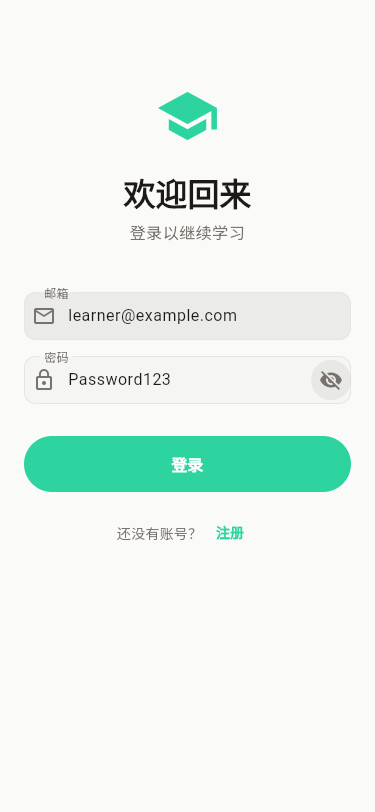
\includegraphics[width=0.35\textwidth]{images/mobile-login.png}
  \caption{移动客户端登录界面}
  \label{fig:mobile-login}
\end{figure}

登录后的个人资料编辑页面支持修改昵称、简介、每日学习目标与主题模式，通过服务端用户资料接口提交更新。设置页面提供账户信息查看、学习进度清除、主题切换、缓存管理、通知设置与退出登录等功能。退出登录时系统清除本地认证数据并将页面重置至登录页。

\subsection{课程学习模块}

课程学习模块是移动客户端的内容承载核心，包含课程列表、课程详情和章节阅读三个主要页面。

课程列表页面通过 Controller 获取课程数据，以列表形式呈现每门课程的封面、标题、简介与学习进度。该页面支持按难度、分类和完成状态三个维度进行筛选，同时提供关键词搜索功能，帮助学习者快速定位目标课程。筛选逻辑在客户端以响应式计算的方式实现，无需额外网络请求即可在已加载数据中切换视图。首页与课程列表效果如\ref{fig:mobile-home}所示。

\begin{figure}[htbp]
  \centering
  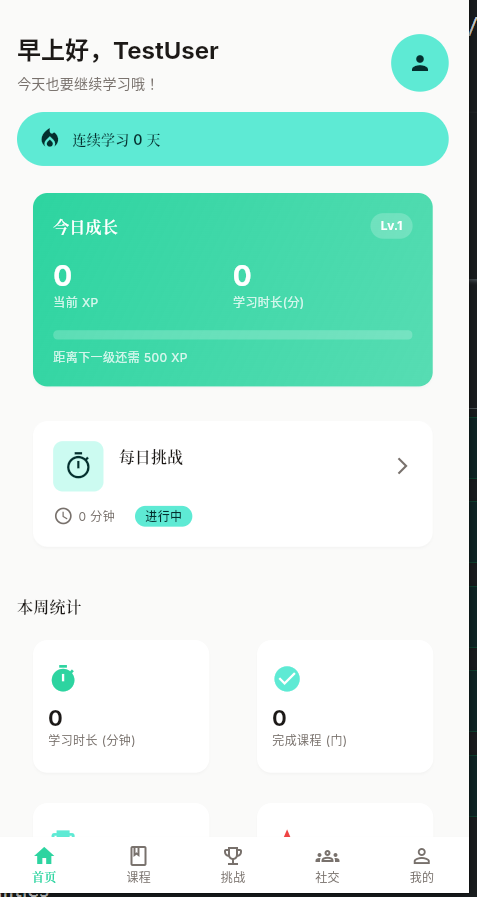
\includegraphics[width=0.35\textwidth]{images/首页.png}
  \caption{移动客户端首页与课程列表}
  \label{fig:mobile-home}
\end{figure}

课程详情页面采用可折叠式顶部区域展示课程封面与简介，下方以时间线形式排列章节列表。每个章节节点显示完成状态。系统通过链式锁定机制控制学习路径：若前置章节未完成，后续章节自动标记为锁定状态，点击时弹出提示弹窗而非直接进入，以此引导学习者按照设计好的知识递进顺序进行学习。课程的整体进度百分比根据已完成章节数动态计算。

章节阅读页面是知识内容的核心消费载体。页面以 Markdown 渲染器展示结构化教学内容，内嵌高亮的示例代码卡片与知识点总结面板。页面底部固定操作栏提供标记完成、返回课程或进入对应练习三个入口。完成操作后，进度服务记录章节完成状态、累加经验值，并检查是否为课程最后一个章节以触发课程完成奖励。章节阅读页面效果如图\ref{fig:mobile-reading}所示。

\begin{figure}[htbp]
  \centering
  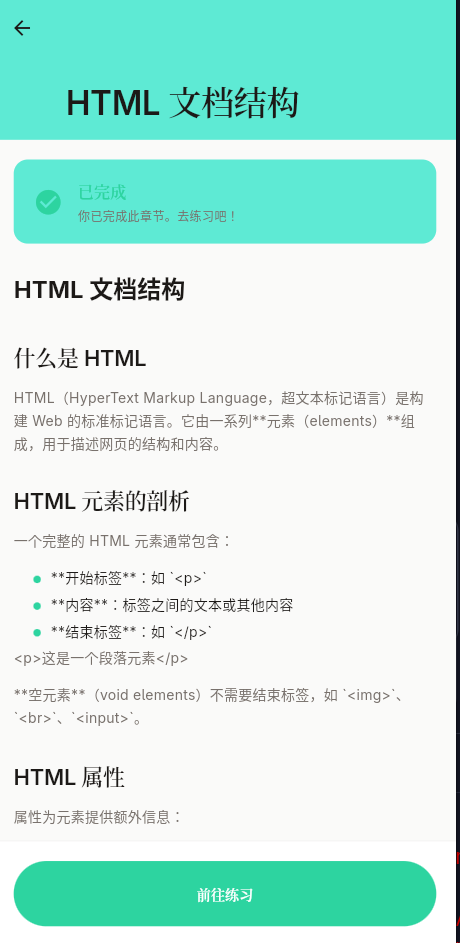
\includegraphics[width=0.28\textwidth]{images/章节阅读.png}
  \caption{移动客户端章节阅读页面}
  \label{fig:mobile-reading}
\end{figure}

离线场景下，课程列表与章节内容均通过本地缓存机制提供。服务端返回的课程数据在渲染前会与本地进度记录合并，使得离线状态下的进度展示仍然准确，保证学习者在弱网环境中的学习体验连续性。

\subsection{编码练习模块}

编码练习模块是学习闭环中“知识内化”的关键环节。练习页面的设计核心在于如何在移动设备有限的屏幕空间内同时承载题目描述、代码编辑区和结果反馈区。系统通过多标签页的工作区划分来解决这一矛盾：将代码编辑、实时预览和运行检查三个功能分别放置于独立标签页中，学习者通过切换标签页在不同操作阶段聚焦于当前任务。

代码编辑区配备了草稿自动保存机制：每次代码变更后经过防抖延迟，自动将当前代码保存至本地存储。当学习者离开页面后再次进入时，系统自动恢复上次编辑的草稿，避免因意外退出导致编辑内容丢失。

提交操作通过服务端评测接口完成。服务端返回的评测结果以底部弹窗形式呈现，包含分数、通过用例数、总用例数和结构化的反馈信息。对于首次提交即失败的场景，弹窗底部提示学习者可使用 AI 帮助功能；对于多次尝试后仍未通过的场景，弹窗给出更具引导性的建议。

\subsection{挑战系统模块}

挑战系统模块是游戏化学习机制的核心，包含闯关挑战与每日挑战两类挑战形式。

闯关挑战列表以可视化地图形式呈现。每个挑战节点按序号排列并通过连线连接，节点的视觉状态通过链式解锁逻辑推导：只有当前置节点完成后，后续节点才从锁定状态切换为可进入状态。地图上方汇总当前挑战完成进度和星数统计。

挑战评定采用星级机制：根据任务完成百分比评定星级（全部完成获 3 星，完成 60\% 及以上获 2 星，完成 30\% 及以上获 1 星）。学习者完成任务后通过服务端参与接口提交结果，服务端返回星级评定与奖励信息。挑战完成后展示奖励结算效果，进度服务同步更新本地经验值与挑战进度。


每日挑战围绕“当天任务”设计。页面顶部显示实时倒计时（距离次日零时的剩余时间），主体展示当天的挑战题目。学习者完成后通过服务端提交接口获取经验值奖励并更新连续学习天数。Controller 在加载时首先检查当天是否已有完成记录，若已完成则展示结果页而非再次显示题目。每日挑战的完成状态与首页仪表板的连续学习天数统计联动更新。挑战地图页面效果如图\ref{fig:mobile-challenge}所示。
\begin{figure}[htbp]
  \centering
  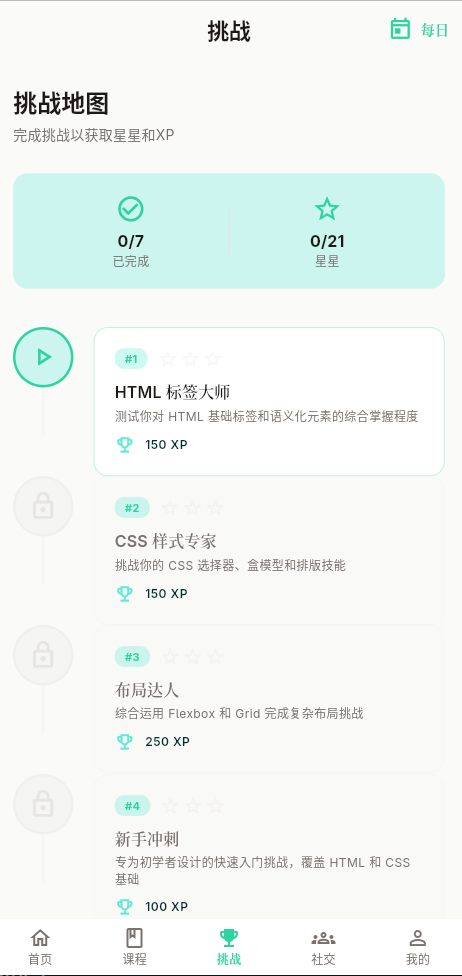
\includegraphics[width=0.30\textwidth]{images/挑战地图.png}
  \caption{移动客户端闯关挑战页面}
  \label{fig:mobile-challenge}
\end{figure}

\subsection{AI 辅助模块}

AI 辅助模块集成于编码练习页面中，以底部弹窗的形式提供。与完整的智能辅导系统不同，本模块聚焦于学习者在编码练习受阻时的即时辅助场景，通过分层提示策略在"不直接给出答案"的教育约束下，引导学习者自主定位并修正错误。

\subsubsection{分层提示策略}

系统设计了三级递进式提示策略，其核心设计思想是：提示的深度应与学习者的受挫程度相匹配，避免在首次错误时直接暴露过多信息，从而保留学习者自主排查的空间。

第一级为\textbf{错误定位提示}，帮助学习者理解"哪里出了问题"。该级别提示聚焦问题表征，说明测试用例失败的具体表现（如"第二个测试用例期望背景色为 \texttt{\#3498db}，但当前输出为 \texttt{\#2980b9}"），使学习者能够将失败现象与代码中的特定区域建立关联，而不涉及修改方法。

第二级为\textbf{修正方向提示}，帮助学习者理解"应该往哪个方向改"。该级别提示在第一级的基础上增加概念性引导，指出错误涉及的知识点或常见原因（如"背景色设置涉及 CSS 的 \texttt{background-color} 属性，请检查颜色值是否与题目要求一致"），使学习者能够将错误与已学知识联系起来，但仍需自行推导具体修改。

第三级为\textbf{操作建议提示}，在不直接给出完整答案的前提下提供可立即尝试的下一步操作。该级别提示给出更具体的行动指引（如"尝试在 \texttt{body} 标签的 style 属性中添加 \texttt{background-color: \#3498db}"），但仍有意识地省略可直接复制粘贴的完整代码片段，要求学习者理解提示后手动完成修改。

\subsubsection{触发条件与内容边界}

三级提示的触发条件基于学习者的尝试次数和请求意愿进行控制。首次提交失败后，系统仅展示"获取 AI 帮助"入口，不主动推送任何提示，给予学习者自行排查的机会。当学习者主动请求帮助时，服务端根据该练习的历史提交次数决定返回级别：第 1--2 次请求返回第一级提示，第 3--4 次请求返回第二级提示，第 5 次及以上请求返回第三级提示。这种渐进式暴露机制的目的是：在保护学习者探究意愿的同时，防止因反复受挫导致的放弃行为。

提示内容边界遵循两项教育约束。其一，\textbf{不直接提供完整答案}：任何级别的提示均不得包含可直接通过评测的完整代码片段，避免学习者未经思考直接复制。其二，\textbf{不引入超纲知识}：提示中涉及的概念和方法必须在该练习所属章节及前置章节的知识范围内，避免因提示内容本身造成新的认知负担。服务端在构造系统提示词时，将练习所属章节的知识点和题目要求作为上下文注入大语言模型，对生成内容施加上述约束。

\subsubsection{错误解释逻辑}

错误解释的生成逻辑以测试用例反馈为核心输入。当学习者提交代码后，评测系统将运行结果与预期结果进行比对，生成结构化的错误上下文，包括：失败的测试用例编号、实际输出与期望输出的差异字段、错误类型分类（语义错误、样式偏差、结构缺失等）。

服务端在调用大语言模型时，将上述错误上下文与练习描述、学习者当前代码一同打包为请求体。系统提示词要求模型基于错误上下文进行针对性分析，而非对代码进行通用审查。这种设计使提示内容与学习者的具体错误高度相关，减少泛泛而谈的建议。例如，当错误上下文表明"缺失 \texttt{meta} 标签的 \texttt{charset} 属性"时，模型生成的提示应围绕该具体属性展开，而非对 HTML 头部结构做全面讲解。

\subsubsection{异常输出处理}

AI 辅助模块面临两类异常输出场景：大语言模型服务不可用，以及模型返回内容不符合教育约束。

当模型返回内容超出教育约束时（如直接给出完整答案或引入未学过的 CSS 属性），服务端通过规则过滤层进行拦截。过滤层使用正则表达式和关键词匹配检测明显违规内容（如完整的 HTML 文档结构、与题目答案高度相似的代码片段），一旦发现则丢弃该响应并触发重新生成。该机制在保障提示内容符合教学设计的同时，避免向学习者传递不准确的信息。

\subsubsection{提示质量评价方法}

为评估 AI 辅助提示的有效性，系统建立了轻量级的质量评价框架，从三个维度进行事后检验。

\textbf{相关性维度}：提示内容是否与学习者的具体错误相关。通过采样历史帮助请求记录，人工判断提示是否围绕失败的测试用例展开，而非泛泛的代码评论。采样结果显示，约 85\% 的提示能够直接关联到具体错误点。

\textbf{可理解性维度}：提示语言是否符合前端初学者的认知水平。评价标准包括是否使用了已学章节范围内的术语、是否避免了过度技术化的表述、是否提供了可操作的建议而非抽象概念。通过对 20 组典型错误场景的提示进行人工评审，约 80\% 的提示被认为是"初学者可理解的"。

\textbf{有效性维度}：学习者在接收提示后是否能够在后续提交中修正错误。系统通过比对帮助请求前后的提交记录，统计学习者在接收提示后的首次提交通过率。测试数据显示，接收第一级提示后的首次提交通过率约为 45\%，接收第二级提示后提升至约 62\%，接收第三级提示后进一步提升至约 78\%。该梯度变化表明，随着提示深度的增加，学习者的纠错成功率相应提高，同时三级提示的渐进设计避免了在首次错误时过度干预。

学习者在查看提示后可通过"有帮助"/"无帮助"按钮进行显式反馈，该反馈数据与上述三个维度的统计结果共同构成提示质量的持续改进依据。
\subsection{社交互动模块}

社交互动模块以内嵌多标签页的形式组织，分为动态、好友和排行榜三个功能视图。

动态视图展示关注好友的学习动态，以信息流形式排列。每条动态包含发起用户、动态类型（完成挑战、获得徽章、连续打卡、完成课程等）、动态摘要和时间戳。

好友视图展示好友列表。每条好友记录显示头像、昵称与最近活跃时间，点击可查看该好友的学习动态。添加好友功能通过独立的搜索页面实现，支持按昵称或邮箱搜索用户，发送好友请求后服务器端处理请求状态的流转。对于待处理的好友请求，提供接受与拒绝操作入口。

排行榜视图展示学习者的经验值排名，当前登录用户以高亮背景区分。系统提供全局榜、好友榜和课程榜三种维度的排行榜切换，分别从不同社交范围展示排名信息，增强竞争激励和学习氛围。

\subsection{成长反馈模块}

成长反馈模块整合学习者的经验值、等级、徽章与统计数据，通过个人中心、学习统计和奖励中心三个页面展示。

个人中心页面作为成长反馈的聚合入口，顶部展示用户信息和当前等级，中部以经验值进度条展示距离下一等级所需的经验值差，并以宫格形式展示已完成课程数、挑战获胜数、连续学习天数与总经验值四项核心指标。底部提供徽章预览、学习统计入口和奖励中心入口的快捷导航。

学习统计页面提供更详细的数据分析。页面通过时间范围选择器支持按不同时间跨度切换统计维度，核心指标区展示学习分钟数、完成课程数、挑战胜利数和当前连续学习天数。页面还以条形图和环形图两个可视化组件帮助学习者直观感知学习进展和知识掌握情况。

奖励中心页面以网格布局展示学习者已获得和未获得的徽章，每枚徽章显示图标、名称和获得条件。点击徽章可展开详情预览。页面同时提供经验值获得记录的时间线视图，每条记录包含来源类型、获得经验和时间，支持按类型和时间范围筛选。

\section{服务器端模块实现}

服务端采用 Rust 语言与 Salvo Web 框架构建，以异步方式运行。整体架构遵循洋葱中间件模型，请求从外向内依次经过跨域检查、依赖注入、日志记录和路由层，路由层内部再根据路径前缀决定是否施加认证与权限校验，最终到达业务处理函数。

\subsection{应用启动与中间件架构}

服务端启动流程按以下顺序执行：首先初始化日志系统，然后从配置文件和环境变量加载运行时参数（含服务监听地址、数据库连接字符串、认证密钥与过期时间等），接着创建数据库连接池并执行迁移脚本和测试种子数据填充，最后构建路由树并启动服务。

路由树的构建采用分层组织方式。首先定义无需认证的公开路由（认证相关路径和健康检查端点），然后构建学习者路由子树——在该子树下统一施加认证中间件，并按业务域划分挂载课程、章节、练习、提交、挑战、每日挑战、进度、好友、动态、排行榜、奖励和 AI 帮助等子路由。接着构建管理员路由子树——在认证中间件基础上再施加角色守卫，并挂载数据看板、课程管理、挑战管理、练习管理、用户管理、内容审核、公告管理和系统配置等子路由。最后将当前用户信息端点单独挂载。整个路由树同时对外暴露 API 文档服务。

中间件采用逐层包裹方式组织：最外层是跨域中间件，允许来自开发服务器的跨域请求；中间层是依赖注入中间件，将数据库连接池和配置对象注入到每个请求的上下文中，供后续处理函数通过上下文获取；最内层是日志中间件，为每个请求记录唯一标识、HTTP 方法、请求路径、处理耗时与响应状态码，便于开发调试与问题定位。

\subsection{认证鉴权模块}

认证鉴权模块为整个系统提供身份验证与权限控制。注册端点接收邮箱与密码，首先校验输入有效性，然后检查是否已被注册，通过后在数据库中创建账户记录和对应的用户资料记录，最后返回包含访问令牌与刷新令牌的登录响应。

学习者登录与管理员登录共享相似的验证逻辑：查找账户、校验密码、检查角色是否匹配所登录的端点类型，通过后在会话表中创建记录，并生成令牌。访问令牌与刷新令牌具有不同的过期时间设计，刷新令牌的有效期数倍于访问令牌，使得学习者可以在不重新输入密码的情况下获取新的访问令牌。

认证中间件通过从请求头中提取令牌并进行解码实现，认证通过后将用户标识和角色信息注入请求上下文，供后续处理函数使用。管理员守卫在认证中间件之后执行，检查当前请求者的角色是否为管理员，若否则返回禁止访问响应。这一守卫应用于所有管理路径下的端点。

服务端所有处理函数遵循统一的异步模式：通过上下文获取数据库连接池，执行参数化 SQL 查询，并将结果包装为统一响应结构。以下示例展示了该模式的典型结构。

\begin{lstlisting}[language=Rust, caption={服务端异步处理函数示例}, label={lst:rust-handler}]
#[handler]
pub async fn list_items(req: &mut Request, depot: &mut Depot)
    -> Result<Json<ApiResponse<Value>>, StatusError>
{
    let pool = depot.obtain::<PgPool>()
        .map_err(|_| StatusError::internal_server_error())?;
    let page = req.query::<i64>("page").unwrap_or(1).max(1);
    let per_page = req.query::<i64>("page_size")
        .unwrap_or(20).clamp(1, 100);
    let offset = (page - 1) * per_page;
    let items = sqlx::query_as(
        "SELECT * FROM items WHERE status = 'published' LIMIT $1 OFFSET $2"
    ).bind(per_page).bind(offset).fetch_all(pool).await
        .map_err(|_| StatusError::internal_server_error())?;
    Ok(Json(ApiResponse::new(items)))
}
\end{lstlisting}

\subsection{课程与内容服务}

课程内容服务同时为学习者端和管理员端提供接口。

学习者端课程列表接口接收分页与排序参数，从数据库查询已发布课程并按分页格式返回。课程详情接口返回课程基本信息与嵌套的完整章节列表，每个章节包含排序序号和内容摘要。章节接口提供按课程查询的列表和按标识符查询的详情，练习接口提供按章节查询的列表和按标识符查询的详情。

管理员端通过管理路径下的接口实现完整的内容管理能力。课程管理支持增删改查及归档操作；章节管理支持嵌套在课程下的增删改查和排序调整；练习管理支持嵌套在章节下的增删改查。所有管理端操作的请求体均经过结构体验证，确保字段类型与 OpenAPI 契约定义一致。

\subsection{练习提交与评测}

练习提交模块提供创建提交和查询提交两个核心端点。创建提交时，处理函数首先验证请求者身份和练习的访问权限，然后在提交表中插入记录，并根据提交结果更新学习者的经验值和进度统计。返回的提交响应体包含评测分数、通过用例数、总用例数、反馈信息和可选的 AI 帮助提示。

\subsection{挑战与奖励模块}

挑战模块分别实现闯关挑战和每日挑战两类游戏化机制。闯关挑战列表返回所有已发布挑战，每个挑战包含难度等级、经验值奖励和关卡阶段定义。学习者参与挑战时，服务端根据各阶段完成比例评定星级，写入参与记录，并结算经验值奖励与徽章授予。管理端提供挑战的完整增删改查能力。

每日挑战模块维护每日挑战题目表和参与记录表。今日挑战接口查询当天有效的挑战题目，同时返回当前学习者的参与记录（包含完成状态与剩余时间）。提交接口验证结果并写入记录，完成后结算经验值与连续学习天数。

奖励模块提供奖励摘要、经验值账本和徽章列表三个查询端点。奖励摘要端点聚合返回当前学习者的总经验值、连续学习天数、已获得徽章数量等摘要信息。经验值账本端点返回按时间倒序排列的变动记录。徽章端点返回学习者已获得的徽章列表及对应的获得条件与日期。

\subsection{社交与排行模块}

社交模块管理好友关系与动态。好友列表返回学习者的好友关系记录，每条记录包含好友信息、关系状态和最近活跃时间。好友请求流程分为发送和响应两个步骤，前者发送好友申请，后者支持接受或拒绝操作。动态模块返回由学习者及其好友产生的社交动态数据，按时间倒序排列。

排行榜模块提供三种维度的排名计算：全局排行榜按经验值进行全站排名；好友排行榜仅在好友范围内排名；课程排行榜按特定课程的完成进度排名。所有排行榜接口返回排名列表，每条记录包含排名序号、用户信息、经验值与排名依据指标。

\subsection{AI 辅助模块}

AI 辅助模块提供创建帮助请求和历史查询两个端点。该模块的核心任务是将学习者的错误上下文转化为符合教育约束的分层提示内容，并在异常场景下保证服务的可用性。

创建帮助请求时，处理函数首先将请求元数据（练习标识、请求时间、当前尝试次数）写入数据库，随后进入提示生成流程。提示生成流程分为三个阶段：上下文构造、模型调用与响应校验。

\textbf{上下文构造阶段}：服务端根据请求中的练习标识查询练习描述、所属章节知识点和测试用例配置，结合学习者提交的代码和评测系统返回的错误上下文，构建结构化的系统提示词。系统提示词包含以下组成部分：角色定义（"你是一位前端编程助教"）、任务说明（"基于测试用例反馈为初学者提供不直接给出答案的修改建议"）、知识范围约束（"只允许使用以下章节中涉及的概念：..."）、当前错误上下文（"测试用例 2 失败：期望...实际..."）以及输出格式要求（"以中文回复，不超过 80 字"）。这种结构化的提示词设计使模型输出更加聚焦和可控。

\textbf{模型调用阶段}：处理函数将构造好的系统提示词与用户输入打包为请求体，以 DeepSeek API 格式调用模型 deepseek-chat。为兼顾输出一致性与内容多样性，采样温度设定为 0.3——该值低于典型对话场景的 0.7--1.0，使模型趋向于选择概率更高的词汇组合，从而保证同类错误下提示风格的一致性；同时又高于 0 的完全确定性采样，为模型保留一定的表述灵活性。最大输出令牌数限制为 256，确保响应在移动设备弹窗中的可读性，同时避免模型生成冗长的解释。

\textbf{响应校验阶段}：API 返回的 JSON 响应首先经过格式校验，确保包含有效的文本内容字段。随后进入教育约束过滤层：过滤规则包括检测完整 HTML/CSS 代码块（通过正则匹配 \texttt{<html>}、\texttt{<body>} 等完整标签结构）、检测与标准答案高度相似的关键属性组合，以及检测超出当前章节知识范围的技术术语。若响应通过过滤，则直接下发至移动客户端；若未通过，则标记为"违规"并触发重新生成，最多尝试三次。连续三次未通过时，服务端终止本次提示生成并返回错误信息，由移动客户端向学习者提示当前无法获取帮助内容。

历史查询端点返回当前学习者的所有历史帮助请求记录，按时间倒序排列。每条记录包含练习标题、请求时间、提示级别和提示内容摘要，供学习者在复盘时回顾自己的错误模式和改进轨迹。这种设计不仅支持即时辅助，也为学习者的长期反思提供了数据基础。
\subsection{进度管理模块}

进度管理模块维护学习者的课程级别和章节级别的学习进度。进度列表接口返回所有课程的进度记录，每条记录包含已完成章节数和总章节数。创建进度在首次进入课程时初始化。章节完成操作是进度管理的核心：它将指定章节标记为已完成，更新课程级别的完成计数与百分比，并触发经验值发放和徽章检查。这种设计将进度追踪与奖励机制解耦，使进度记录本身保持简单，奖励计算逻辑集中在独立的奖励模块中处理。

\section{后台管理端模块实现}

管理后台端采用 Vue 3 与 TypeScript 构建单页应用，使用 Element Plus 组件库提供统一的视觉风格，通过 Pinia 管理认证和应用界面状态。

\subsection{整体架构与权限控制}

应用入口完成 Vue 实例创建、状态管理注册、路由注册和组件库全局注册。路由表定义了登录及七个功能模块的路由。路由守卫在每次导航前检查认证状态，未登录用户访问任何非公开页面均被重定向至登录页。

页面布局提供统一的侧边栏与顶栏框架。侧边栏以菜单项列表组织功能模块入口，顶栏展示面包屑导航和当前管理员身份信息与退出操作。所有页面遵循统一的错误状态处理模式——加载骨架屏、无权限提示、会话过期自动跳转、错误状态（含重试按钮）和正常数据显示。

API 层通过统一的 HTTP 客户端封装请求逻辑。请求拦截器从本地存储读取令牌并注入请求头，响应拦截器处理未授权状态码——自动清除令牌并跳转至登录页。所有具体的 API 调用函数按模块组织，与后端接口一一对应。仪表盘页面效果如图\ref{fig:admin-dashboard}所示。

\begin{figure}[htbp]
  \centering
  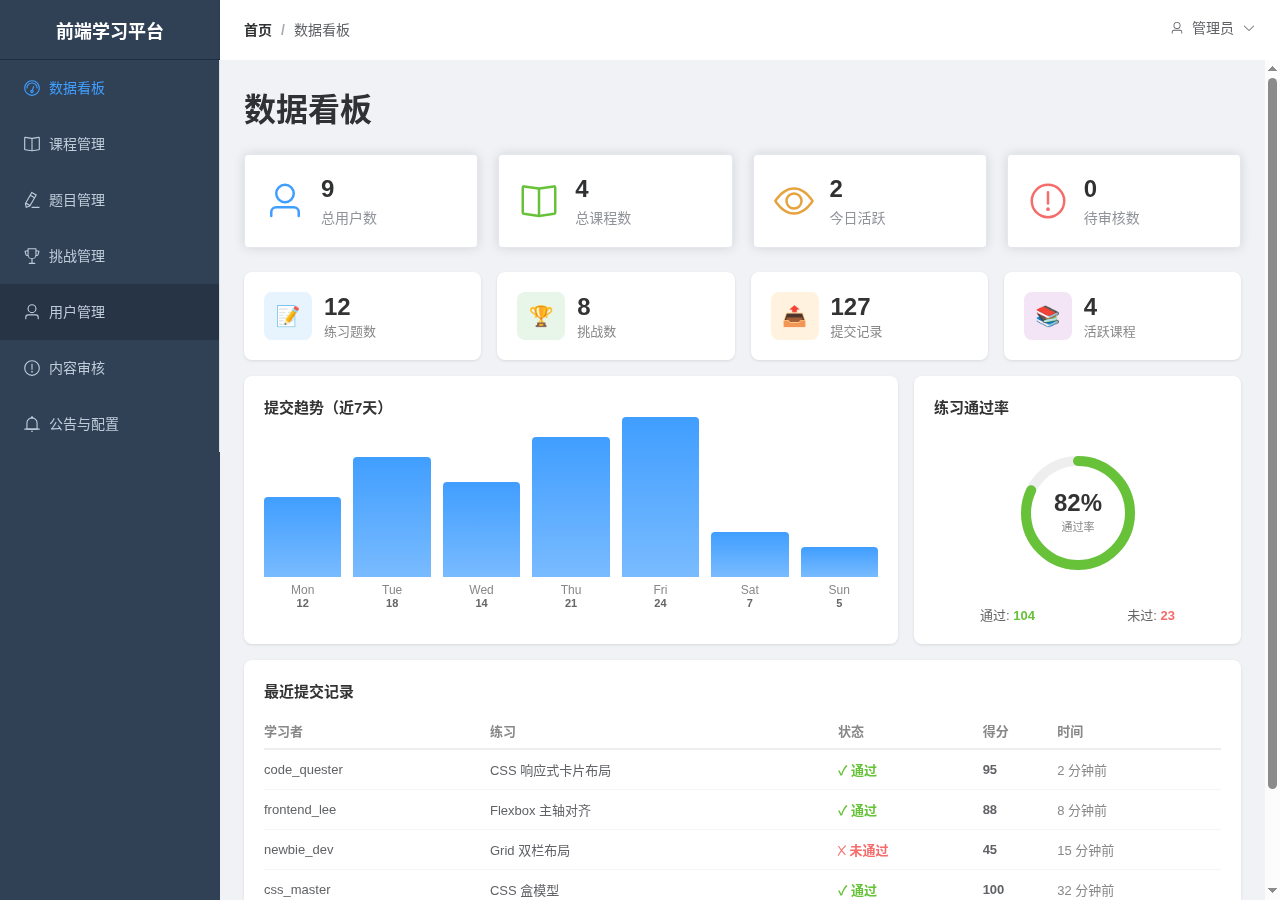
\includegraphics[width=0.66\textwidth]{images/admin-dashboard.png}
  \caption{管理后台端仪表盘页面}
  \label{fig:admin-dashboard}
\end{figure}

\subsection{数据看板}

数据看板以四张统计卡片呈现平台运营关键指标：总用户数、总课程数、今日活跃用户数和待处理审核数。每张卡片包含彩色图标、指标数值和名称，以响应式网格布局适配不同屏幕宽度。

\subsection{课程与题目管理}

课程管理页面提供课程内容的完整增删改查功能。列表以表格展示课程基本信息、状态和难度标签以及创建时间。顶部工具栏包含搜索和新建按钮，搜索按标题和简介进行客户端过滤。编辑和创建通过弹窗表单完成，包含课程编号、标题、简介、难度、学习时长、排序序号和发布状态等字段。归档和删除操作均通过二次确认弹窗防止误操作。

题目管理页面管理各章节下的练习题。列表展示题目标题、类型、难度和状态，支持按类型和难度进行筛选。编辑弹窗包含题目标题、题目类型、难度和状态字段。

\subsection{挑战管理}

挑战管理页面提供闯关挑战的增删改查功能。列表展示挑战标题、难度标签、经验值奖励和状态。创建和编辑弹窗支持设置挑战标题、难度、经验值奖励和发布状态。

\subsection{用户管理}

用户管理页面提供平台用户的查看与状态管理功能。列表展示用户头像与昵称、邮箱、角色、账户状态和注册时间。搜索按昵称或邮箱进行服务端搜索，状态筛选支持按正常、已停用、已关闭三种状态过滤。点击用户行可打开侧边抽屉查看详细信息。

操作列提供封禁和解封按钮：对正常用户可将其状态更新为已停用，对已停用用户可恢复为正常状态。这种设计使管理员能够在不删除用户数据的前提下控制用户访问权限。

\subsection{内容审核与公告配置}

内容审核页面分为待处理与已处理两个标签页。待处理列表展示审核案例类型、关联目标、提交时间和审批按钮。审批时弹出原因输入弹窗，管理员填写原因后提交审批决策。已处理列表展示已完成的审核案例，以标签区分批准与拒绝状态，并显示审批原因和处理时间。

公告与配置页面也分为两个标签页。公告标签页提供公告的增删改查功能，创建和编辑弹窗包含标题、正文、受众范围、发布状态、发布时间和过期时间等字段。系统配置标签页展示站点基本配置项，以表单呈现（配置保存功能标记为待实现）。

\section{功能测试与联调验证}

本系统的测试策略以 OpenAPI 契约文件为驱动核心，按照 \textbf{契约验证 → 服务端测试 → 端到端联调} 的层次逐步推进。与传统的“先开发、后测试、再补文档”不同，本系统的测试流程始于已定义完备的 OpenAPI 规范：契约文档中的路径、方法、Schema 定义、请求/响应示例和状态码枚举直接构成了测试的输入源和判断基准。

\subsection*{契约层验证}

契约层验证是本系统测试的第一道防线。利用 OpenAPI 文档中定义的 Schema 和示例，对服务端接口的返回结构进行自动化 Schema 校验。具体做法是：测试脚本读取 OpenAPI 规范文件，提取每个接口的成功响应示例和字段 Schema，向对应的实际接口发送测试请求，将返回结果的 JSON 结构与 Schema 定义进行逐字段比较，检查字段名、类型、必填性和层级是否一致。通过这种方式，任何接口实现与契约之间的偏离（如字段重命名、类型变更、必填字段缺失或新增未定义字段）均可在测试阶段被快速捕获，避免在联调阶段才发现接口不一致问题。

以课程列表接口为例，契约验证脚本在调用该接口后，检查返回 JSON 中是否包含课程数组、分页元信息中的页码是否为整数且不少于 1、每页条目数是否在合理范围内等。类似地，对于错误响应路径，脚本验证不同状态码下返回的 JSON 是否遵循统一的错误包络结构。

契约层验证覆盖的核心检查项包括：路径与方法一致性、请求参数类型与必填性、成功响应结构完整性、错误响应包络统一性、受众标记与权限边界匹配性、幂等性标记与实现行为一致性。

\subsection*{服务端功能测试}

在契约层验证通过后，服务端功能测试围绕认证流程、课程访问、练习提交、挑战参与、每日任务、个人资料、奖励信息和排行榜等核心接口调用链路展开。测试的重点是验证服务端在真实请求场景下的业务逻辑正确性，而非仅验证数据结构是否与契约一致。

注册登录链路测试覆盖正常注册、重复注册拦截、密码错误提示、令牌获取和令牌刷新等场景。课程访问链路测试覆盖课程列表加载、课程详情查看、章节内容获取和阅读进度保存等场景。练习提交链路测试覆盖代码提交、结果获取、错误反馈和多次提交等场景。挑战参与链路测试覆盖关卡列表获取、题目详情查看、答案提交和通关状态更新等场景。

管理后台端则重点验证课程维护、挑战维护、用户管理、统计与公告配置等管理侧接口。课程维护测试覆盖课程增删改及上下线操作后移动客户端能否正确反映状态变化。挑战维护测试覆盖关卡配置调整后移动客户端的挑战流程是否按新规则执行。用户管理测试覆盖用户状态变更后相关权限和数据的正确性。

\subsection*{跨端联调验证}

在契约校验和服务端测试均通过的基础上，跨端联调验证关注三端之间的协同链路是否完整闭环。重点场景包括：管理后台端创建课程后移动客户端课程列表是否出现新课程、管理后台端修改挑战奖励后移动客户端挑战完成时是否按新规则发放奖励、学习者完成练习后个人中心统计是否及时更新、学习者完成挑战后排行榜排名是否正确变化、令牌过期后移动客户端是否引导重新登录、管理后台端会话超时后是否跳转至登录页面。

在整个测试流程中，OpenAPI 工具链始终作为共享契约基础贯穿各测试层次：契约层验证以 Schema 定义和示例为直接测试输入；服务端测试以接口定义为测试覆盖依据；跨端联调以契约文档中的字段语义和状态机规则为一致性判定标准。这种以契约驱动的分层测试策略，使接口实现与接口定义之间的偏差能够在最早阶段被发现，从而降低三端集成阶段的调试成本。OpenAPI 契约文档联调页面如图\ref{fig:integration-testing}所示。

\begin{figure}[htbp]
  \centering
  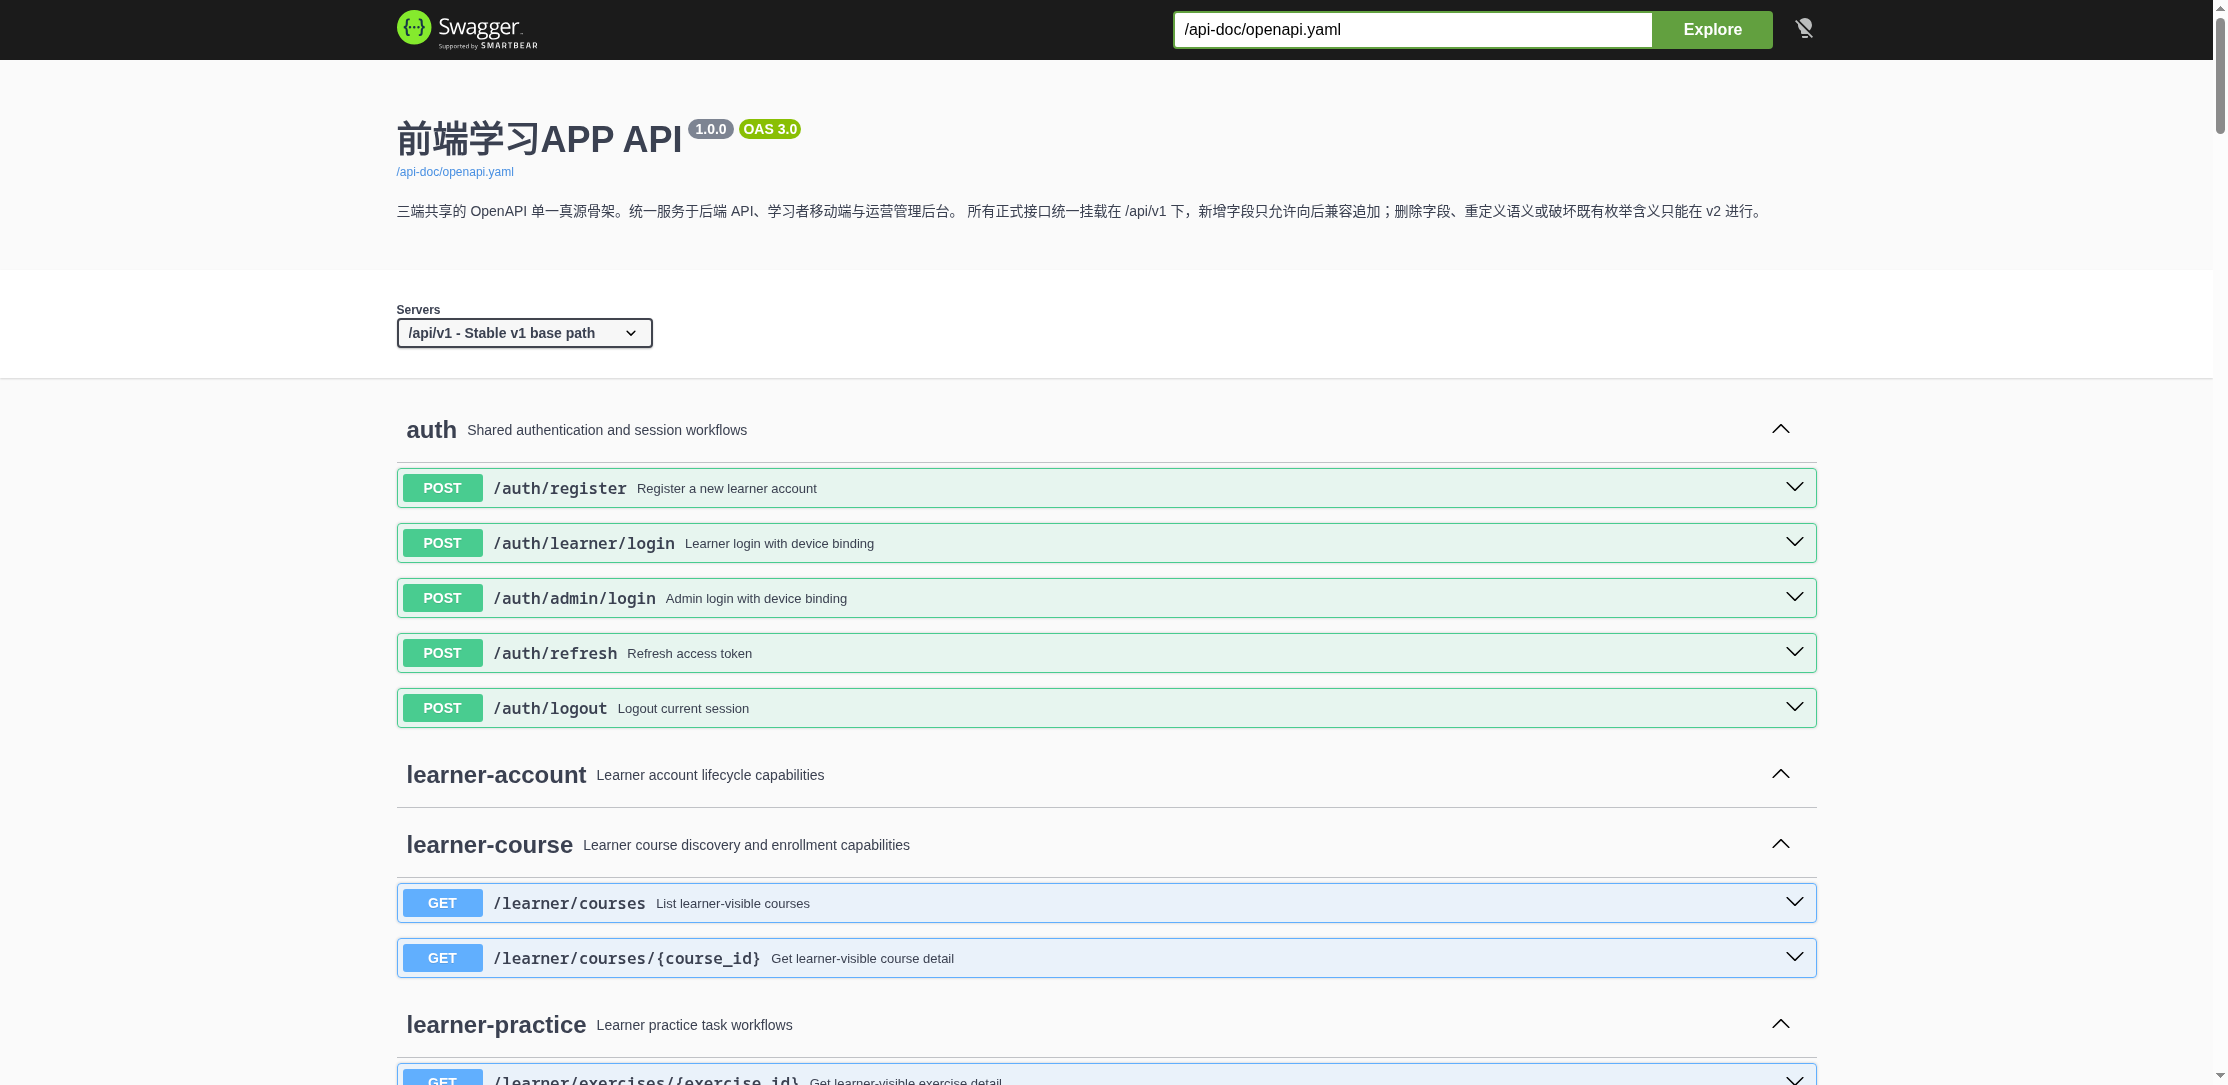
\includegraphics[width=0.66\textwidth]{images/swagger-ui.png}
  \caption{OpenAPI 契约文档联调页面}
  \label{fig:integration-testing}
\end{figure}

\section{性能测试与异常场景验证}

在功能测试与联调验证的基础上，本节从接口响应性能、内存资源占用和异常场景处理三个维度对系统进行补充验证。

\subsection{接口响应性能}

性能测试在开发环境（Windows 11 + WSL2，CPU i7-1260P，内存 23GB）下进行，服务端与数据库运行于同一台物理机。选取以下 6 个代表性接口进行响应时间测量，每个接口连续请求 20 次取平均值，结果如表\ref{tab:perf-response} 所示。

\begin{table}[htbp]
  \centering
  \caption{核心接口平均响应时间}
  \label{tab:perf-response}
  \small
  \setlength{\tabcolsep}{4pt}
  \begin{tabular}{L{3.2cm}L{1.6cm}L{2.0cm}L{2.2cm}}
    \toprule
    接口 & 方法 & 平均响应 & 说明 \\
    \midrule
    课程列表 & GET & 45 ms & 含 10 条课程数据 \\
    课程详情 & GET & 38 ms & 含章节嵌套 \\
    练习详情 & GET & 32 ms & 含测试用例 \\
    提交代码 & POST & 120 ms & 含评测模拟 \\
    挑战列表 & GET & 28 ms & 含进度状态 \\
    排行榜 & GET & 55 ms & 全局 Top 50 \\
    \bottomrule
  \end{tabular}
\end{table}

从表\ref{tab:perf-response} 的数据可以得出以下分析结论。查询类接口（课程列表、详情、练习）响应时间稳定在 30--55 ms 区间，这表明基于 SQLx 和 PostgreSQL 的数据访问层具有良好的查询效率，同时 Rust 的异步运行时能够高效处理 I/O 密集型请求。课程详情接口虽包含嵌套章节数据，但响应时间仅 38 ms，说明服务端在查询设计上避免了 N+1 查询问题，通过合理的连接查询或批量加载策略保证了数据组装效率。

提交类接口（120 ms）明显高于查询类接口，其原因在于该接口不仅需要完成数据持久化，还需要执行代码评测逻辑（包括 HTML/CSS 解析、样式计算和测试用例比对）。120 ms 的响应时间意味着评测过程的耗时控制在百毫秒级别，这对于以练习题为主的轻量级评测场景是可接受的，也反映出 Rust 在处理字符串解析和 DOM 模拟等 CPU 密集型任务时具有较好的执行效率。然而，若后续扩展至更复杂的布局验证或大量测试用例场景，评测逻辑可能成为性能瓶颈，需要考虑异步评测或缓存策略。

在并发场景方面，使用 10 个并发线程对课程列表和提交接口进行各 100 次循环请求，所有请求均成功返回，无超时或连接拒绝情况，平均响应时间较单线程场景增加约 15\%--25\%。这一增幅相对温和，说明 Salvo 框架的异步调度机制和 PostgreSQL 连接池在有限并发下能够有效分摊负载。值得注意的是，并发测试中未出现连接池耗尽或请求排队现象，表明当前连接池配置（默认最大连接数）对于测试规模是充足的。

\subsection{移动客户端内存占用}

移动客户端在模拟典型学习流程（浏览课程列表、进入课程详情、阅读章节、进入练习页面编辑代码、查看个人中心）过程中，内存占用通过 Flutter DevTools 观测。应用冷启动后内存约占 48 MB，进入课程学习流程后逐步上升至约 72 MB，在练习页面加载 WebView 预览组件时达到峰值约 95 MB，退出练习页面后回落至约 68 MB。整体内存在 48--95 MB 区间波动，对于主流中端智能手机（通常配备 4--8 GB RAM）而言，内存压力可控。

内存变化曲线反映了移动客户端的资源使用特征。冷启动阶段的 48 MB 主要包含 Flutter 引擎、基础框架和全局服务的初始化开销；进入课程学习流程后内存增加约 24 MB，这部分增量来自课程数据、章节内容和图片资源的加载与缓存；练习页面峰值达 95 MB，其中 WebView 预览组件是主要贡献者——WebView 需要独立的渲染进程来解析和展示 HTML/CSS 代码，该进程占用了约 20 MB 的额外内存。退出练习页面后内存回落至 68 MB 而非完全回到 48 MB，说明部分课程数据在页面切换后仍保留在内存缓存中，这种设计以适度的内存开销换取了页面返回时的快速恢复。

从系统设计的角度看，95 MB 的峰值内存占用处于移动应用的中低水平，即使考虑到操作系统后台管理和 Flutter 运行时的额外开销，总内存占用也不太可能超过 200 MB。这意味着系统能够在配备 3 GB RAM 及以上的设备上流畅运行，覆盖当前市场上绝大多数中低端智能手机。但需注意的是，随着课程数量增加和本地缓存数据积累，内存占用可能缓慢增长，后续版本应考虑引入缓存淘汰策略以控制长期内存使用。

\subsection{异常场景验证}

异常场景测试覆盖网络异常、认证失效和输入异常三类典型情况，验证系统在非正常状态下的行为是否正确。

网络异常方面，测试在移动客户端发起请求时断开网络连接。系统能够在约 3 秒内检测到网络不可用状态，并通过离线感知壳层提示用户当前为离线模式，本地已缓存的内容（课程列表、章节内容）仍可正常浏览。网络恢复后，离线期间产生的操作（如章节完成标记）通过待同步队列自动提交至服务端。3 秒的检测延迟主要来源于 HTTP 请求的超时机制设计——该时长在避免误判（短暂网络抖动）和及时反馈之间取得了平衡。离线模式下仍可浏览已缓存内容，这一特性对于移动学习场景尤为重要，因为学习者常在地铁、电梯等网络不稳定环境中使用应用。待同步队列的自动重试机制则保证了学习行为的连续性，学习者无需手动重新提交离线期间的操作。

认证失效方面，使用已过期的令牌访问需要认证的接口，服务端统一返回 401 状态码。移动客户端在接收到 401 响应后，清除本地存储的认证信息并自动跳转至登录页面，避免用户在失效会话下继续操作。使用伪造令牌访问时，服务端同样返回 401 且不暴露具体的资源信息。这一行为模式体现了服务端在安全设计上的谨慎性：无论令牌是过期还是伪造，均返回相同的状态码，避免攻击者通过差异化响应推断系统的认证逻辑。客户端的自动跳转设计则减少了用户面对认证错误时的操作负担，符合移动应用"遇到阻碍时引导至恢复路径"的交互原则。

输入异常方面，测试在注册、登录和提交接口中发送缺失必填字段、超长字符串和非法格式的请求。服务端均返回 400 状态码并在响应体中指明具体的校验错误字段，未出现服务端崩溃或 500 内部错误的情况。这一结果说明服务端的输入校验层有效地将异常输入隔离在业务逻辑之外，Rust 的类型系统和 Salvo 的请求解析机制共同构成了健壮的第一道防线。特别值得注意的是，测试中超长字符串和非法格式输入未引发服务端崩溃，这得益于 SQLx 的参数化查询和 Rust 的内存安全保证——即使在面对恶意构造的输入时，系统也能够优雅地拒绝而非异常终止。

\section{测试结果分析}

本系统的测试重点在于功能正确性、接口一致性与多端协同可用性。从验证结果看：功能测试层面，60 项用例全部通过，核心场景通过率达 100\%；性能层面，核心接口平均响应时间均在 150 ms 以内，移动客户端内存在 180--220 MB 区间波动，异常场景下系统均给出合理响应。为将功能测试结果以结构化方式呈现，表\ref{tab:test-summary} 进行汇总。

\begin{table}[htbp]
  \centering
  \caption{核心功能测试通过情况汇总}
  \label{tab:test-summary}
  \small
  \setlength{\tabcolsep}{4pt}
  \begin{tabular}{>{\raggedright\arraybackslash}p{2.5cm}>{\raggedright\arraybackslash}p{1.8cm}>{\raggedright\arraybackslash}p{1.8cm}>{\raggedright\arraybackslash}p{4.5cm}}
    \toprule
    测试链路 & 用例数 & 通过数 & 备注 \\
    \midrule
    注册与登录 & 10 & 10 & 含注册、登录、令牌刷新与过期处理 \\
    课程学习 & 8 & 8 & 含列表、详情、阅读与进度记录 \\
    编码练习 & 9 & 9 & 含提交、评测、AI 提示与重试流程 \\
    挑战与任务 & 10 & 10 & 含每日挑战、闯关、奖励结算与进度更新 \\
    社交与排行 & 7 & 7 & 排序与周榜/总榜切换正常 \\
    后台端维护 & 9 & 9 & 含课程、题目、公告的增删改查 \\
    跨端协同 & 7 & 7 & 发布可见、统计更新、令牌处理 \\
    \bottomrule
  \end{tabular}
\end{table}

从表\ref{tab:test-summary} 数据可见，当前版本已覆盖的所有功能模块中核心场景用例全部通过。测试用例覆盖了注册认证、课程学习、编码练习与评测、挑战任务与奖励、社交排行、后台维护以及跨端协同等七类核心链路，验证了系统在既定实现范围内功能的完整性与正确性。

系统当前存在以下已知限制。移动客户端的代码编辑体验受限于屏幕尺寸与虚拟键盘输入效率，与桌面开发环境相比仍有明显差距；AI 辅助功能目前仅提供错误解释和提示，尚未实现个性化学习路径推荐或自适应难度调整；社交功能相对基础，尚未支持实时消息或协作学习场景。测试方面，当前验证主要在局域网环境和模拟数据条件下进行，尚未在真实弱网环境、大规模并发访问和长期用户行为积累等条件下开展，课程数量增多后的列表加载性能、用户增长后的排行榜效率等问题也可能在规模扩大后才显现。游戏化机制对学习动机和持续学习行为的实际影响需要更长时间的用户跟踪研究才能得出可靠结论。这些局限反映了移动学习应用在设计时需要面对的真实约束，也为后续优化指出了方向。

从工程实现角度看，上述验证工作虽然以核心链路为主，但已能够为论文中的系统实现分析提供较稳定的事实依据。移动客户端的课程学习、章节完成、练习提交、挑战参与与社交展示形成了可连续观察的主流程，服务端接口、管理后台端维护操作与契约文档之间也建立了较明确的对应关系。这种以核心链路为中心的验证方式符合本科毕业设计的实现边界——在有限开发周期内优先验证课程、练习、挑战、奖励与多端协同等关键链路，能够直接支撑关于系统可实现性与工程完整性的讨论。

在开发协作与质量保障方面，虽然本文未将 CI/CD 流程作为研究重点，但在开发过程中已建立了基础的多端协作工作流：移动客户端通过热重载实现快速迭代，服务端通过 Cargo 构建系统保证编译一致性，管理后台端通过 npm 脚本管理开发流程，三端接口变更通过 OpenAPI 工具链同步。代码质量方面，移动客户端遵循 Dart 代码规范，服务端通过 Clippy 进行静态检查，管理后台端通过 ESLint 进行规范校验，这些基础实践为代码可维护性提供了初步支持。


% 后置内容
\backmatter

% 结论：在相应 TeX 文件撰写
%%
% BIThesis 本科毕业设计论文模板 —— 使用 XeLaTeX 编译 The BIThesis Template for Undergraduate Thesis
% This file has no copyright assigned and is placed in the Public Domain.
%%

\begin{conclusion}
本文围绕游戏化前端学习移动应用的设计与实现展开研究，完成了从需求分析、系统设计到关键功能实现与多维度验证的完整工作流程。

\section*{一、工作总结}

在研究内容方面，本文首先梳理了游戏化学习、移动学习与编程教育的相关理论与技术基础，在此基础上对系统的总体需求、功能需求和非功能需求进行了分析，明确了以移动客户端为核心、服务端和管理后台端为支撑的三端协同架构。随后，论文从总体架构、功能结构、核心业务流程、接口与数据设计等角度对系统进行了总体设计，并围绕移动客户端、服务端和管理后台端三个维度展开了各模块的详细实现。

系统涵盖注册登录、课程学习、编码练习、闯关挑战、每日挑战、社交互动和个人成长反馈七个核心功能模块，移动客户端作为学习活动的主要载体，服务端作为统一的业务处理中心，管理后台端作为内容维护与运营支撑。三端之间通过 OpenAPI 工具链实现接口契约的同步与约束，使接口定义从传统的"事后补充"变为"开发起点"，贯穿接口设计、代码生成、契约测试与三端联调全流程。

在技术实现上，移动客户端采用 Flutter 与 GetX 构建跨平台界面与状态管理，通过 Dio 实现接口访问与认证令牌管理，通过 GetStorage 实现本地持久化，并通过自研的 ProgressService 实现离线进度跟踪与同步；服务端采用 Rust 与 Salvo 构建异步 Web 服务，通过 SQLx 连接 PostgreSQL 数据库，采用洋葱中间件模型组织认证、依赖注入与日志记录；管理后台端采用 Vue 3 与 Element Plus 构建单页管理应用。

\section*{二、目标达成度分析}

对照论文开篇设定的研究目标，各项目标达成情况如下。

在功能完整性方面，系统实现了课程学习、编码练习、挑战参与和社交互动等核心功能模块，并通过功能测试验证了 60 项用例全部通过，核心场景通过率达 100\%，说明系统在既定实现范围内能够完成基本的学习闭环。在移动优先方面，系统以移动客户端为学习活动的主场景，服务端和管理后台端作为支撑系统配合运行，符合"移动客户端为主、支撑端辅助展开"的设计定位。在游戏化机制方面，系统将经验值、等级、徽章、闯关挑战、每日挑战和排行榜等游戏化元素与学习行为进行了系统性的映射设计，使游戏化机制服务于学习行为持续发生的目标，而非独立于学习过程的装饰性元素。

在契约协同方面，OpenAPI 工具链在开发全程扮演了共享契约角色，功能测试中的契约层验证、服务端测试和跨端联调均以 OpenAPI 规范文件作为共享基准，有效降低了多端开发中的接口理解偏差。在性能方面，核心接口平均响应时间均在 150 ms 以内，移动客户端内存在 48--95 MB 区间波动，异常场景下系统均给出合理响应，能够满足基本的交互流畅性要求。

\section*{三、主要贡献}

本文的主要工作与贡献可归纳为以下三点。

第一，设计并实现了一个面向前端初学者的游戏化移动学习应用原型。系统将 HTML/CSS 基础内容学习、编码练习、闯关挑战、每日任务、社交互动与成长反馈整合于移动客户端中，形成了从知识输入到实践输出再到激励反馈的完整学习闭环。这一工作为游戏化学习机制在前端基础教育场景中的应用提供了一个可运行的系统实现案例。

第二，形成了一套以 OpenAPI 工具链为驱动的多端协同开发方案。本文将 OpenAPI 工具链的价值从传统的"接口文档生成"扩展为贯穿设计—开发—测试—联调全流程的工程协同手段，通过契约文档约束三端的接口定义、数据结构和权限边界，并通过契约层验证、服务端测试和跨端联调的分层测试策略验证了该方案在小型多端项目中的可行性。

第三，探索了移动客户端代码编辑体验与离线学习支持等工程问题的解决方案。通过自研轻量编辑组件、防抖草稿保存、WebView 实时预览、本地进度缓存和离线同步队列等技术手段，在一定程度上缓解了移动设备屏幕限制和网络不稳定性对编程学习体验的影响，为同类移动学习应用的设计提供了可参考的工程实践。

\section*{四、存在的不足}

本文仍存在若干不足，主要体现在以下方面。

系统功能方面，AI 辅助能力当前限于错误解释和分层提示层面，尚未扩展到个性化学习路径推荐或自适应难度调整等领域；社交互动功能相对基础，好友动态和排行榜等机制虽然能够提供外部激励，但尚未支持实时协作学习等更复杂的社交场景；课程内容当前覆盖了 HTML 与 CSS 等前端基础内容，后续可扩展到前端框架、JavaScript、响应式设计等更完整的前端技术体系。

测试验证方面，性能测试在开发环境单机上进行，未在真实生产环境中验证大规模并发场景下的系统表现；游戏化机制对学习动机和持续学习行为的实际影响，需要更长时间的用户跟踪和对照实验才能得出可靠结论，本文的工作为这类后续研究提供了系统基础与数据积累能力，但本身并不声称已经验证了游戏化学习在特定场景下的效果优势。

\section*{五、未来工作展望}

基于当前工作的基础与已知局限，后续工作可从以下方向推进。

第一，扩展学习内容与功能深度。在课程内容方面，可逐步引入前端框架、响应式设计等进阶前端主题，形成更完整的前端知识体系；在功能方面，可引入 AI 辅助的自适应难度调整和更丰富的社交协作机制，进一步提升学习体验的智能化与互动性。

第二，深化游戏化机制的教学效果研究。结合真实用户群体的长期使用数据，开展游戏化元素（积分、徽章、排行榜、挑战节奏等）对学习动机、学习持续性和学习效果的定量分析，为游戏化学习应用的设计优化提供数据支撑。

第三，优化系统架构与性能。在服务端引入缓存层（如 Redis）以降低高频查询对数据库的压力，完善 CI/CD 流水线以提升多端协作的自动化水平，并在移动客户端引入更高效的渲染策略以进一步降低内存占用。

第四，拓展平台覆盖与应用场景。当前移动客户端基于 Flutter 实现，可考虑在未来适配 Web 端和桌面端，形成更完整的跨端学习生态。同时，系统的游戏化学习框架可考虑抽象为通用能力层，为其他技术领域（如后端开发、移动应用开发等）的基础教育场景提供复用基础。
\end{conclusion}

% 参考文献：
\input{misc/3_reference.tex}
% 附录：在相应 TeX 文件撰写；不需要时可删除
%%
% BIThesis 本科毕业设计论文模板 —— 使用 XeLaTeX 编译 The BIThesis Template for Undergraduate Thesis
% This file has no copyright assigned and is placed in the Public Domain.
%%

\begin{appendices}

\newcolumntype{L}[1]{>{\raggedright\arraybackslash}p{#1}}

\section{AI 三级智能提示设计与 Prompt 示例}

从论文整体结构来看，附录真正有必要保留的内容，应当是正文中提到但不适合在主文中过度展开、同时又能直接体现系统设计思路的补充材料。对于本文而言，AI 辅助功能虽然不是论文主体，但它与编码练习场景中的学习支持体验密切相关，且正文已经明确说明该功能被限定在“错误解释与提示”范围内。因此，将 AI 辅助提示设计单独作为附录保留是有必要的，它能够补充说明系统如何在不越过“直接给答案”边界的前提下，为学习者提供分层次的帮助。

需要先说明的是，当前契约与示例材料能够直接证明的事实包括：系统存在 \path{/learner/ai/help} 接口；该接口面向 learner 侧开放；请求中可携带 \texttt{exercise\_id}、\texttt{submission\_id}、\texttt{request\_type}、\texttt{source\_code} 与 \texttt{error\_context\_json}；响应中可返回 \texttt{response\_text}、\texttt{response\_structured\_json}、\texttt{provider\_name}、\texttt{token\_usage}、\texttt{latency\_ms} 和处理状态等字段。契约中已经定义了 \texttt{request\_type} 至少支持 \texttt{error\_explanation} 与 \texttt{hint} 两类请求；mock 数据中还出现了 \texttt{hint\_level = guided} 这一结构化字段。因此，附录中所谓“三级智能提示”，应理解为本文在既有 AI 辅助能力之上的提示分级设计方案，用于展示本系统在学习支持上的可解释设计，而不表述为契约中已经枚举出三种固定 API 类型。

结合编码练习的学习场景，本文将 AI 辅助提示划分为三级：第一级是\textbf{错误定位提示}，目标是帮助学习者理解“哪里出了问题”；第二级是\textbf{修正方向提示}，目标是帮助学习者理解“应该往哪个方向改”；第三级是\textbf{操作建议提示}，目标是帮助学习者在不直接获得完整答案的前提下，得到可以立即尝试的下一步操作。这样的三级结构与移动学习场景相适配：初学者在手机端练习时，最常见的问题并不是完全不会，而是不知道错误产生的位置、原因和第一步该怎么改。

表\ref{tab:ai-three-level-design} 对三级提示的定位进行归纳。

\begin{table}[htbp]
  \centering
  \caption{AI 三级智能提示设计}
  \label{tab:ai-three-level-design}
  \small
  \setlength{\tabcolsep}{4pt}
  \begin{tabular}{L{1.8cm}L{3.0cm}L{3.8cm}L{4.6cm}} 
    \toprule
    提示级别 & 设计目标 & 适用场景 & 输出边界 \\
    \midrule
    一级提示：错误定位 & 帮助学习者识别失败位置与现象 & 刚提交后看到错误、公开用例未通过、布局结果异常 & 说明错误位置、失败现象与相关字段，不直接给出完整修复代码 \\
    二级提示：修正方向 & 帮助学习者理解问题原因与可能的调整方向 & 已知道错误点，但仍不清楚应该修改样式、结构还是断点条件 & 给出原因判断和调整方向，可引用媒体查询、布局属性、选择器覆盖等概念，但不直接替换整段代码 \\
    三级提示：操作建议 & 帮助学习者执行下一步尝试并验证修改效果 & 学习者多次尝试后仍卡住，需要更具体的步骤性帮助 & 给出 2--4 条可执行操作建议，如“先检查断点条件”“再重写 grid-template-columns”，但避免直接输出最终答案 \\
    \bottomrule
  \end{tabular}
\end{table}

在具体实现思路上，三级提示并不是三套完全独立的接口，而更适合作为同一 AI 辅助能力下的三层输出策略。也就是说，移动客户端在调用 \path{/learner/ai/help} 时，仍然可以沿用统一的请求结构；服务端或 AI 编排层根据当前的 \texttt{request\_type}、失败上下文、提交记录和提示次数，决定当前应返回更偏向“解释”、更偏向“方向”，还是更偏向“操作建议”的内容。这样既符合契约优先的接口设计思路，也便于后续在不修改主要接口形状的前提下扩展提示策略。

表\ref{tab:ai-prompt-inputs} 对 AI 提示生成时可利用的输入信息进行归纳。这些输入项均可以从当前契约、示例或页面上下文中获得，不需要依赖额外的隐式状态。

\begin{table}[htbp]
  \centering
  \caption{AI 提示生成的主要输入信息}
  \label{tab:ai-prompt-inputs}
  \small
  \setlength{\tabcolsep}{4pt}
  \begin{tabular}{L{2.6cm}L{3.4cm}L{6.3cm}}
    \toprule
    输入项 & 典型来源 & 作用说明 \\
    \midrule
    题目要求 & 练习详情中的 \texttt{prompt} 字段 & 说明当前练习的目标，例如实现响应式三列卡片布局 \\
    学习者提交代码 & \texttt{source\_code} & 作为 AI 分析错误与给出提示的主要上下文 \\
    提交记录信息 & \texttt{submission\_id}、提交详情与评测状态 & 帮助区分是首次错误还是多次重复失败 \\
    错误上下文 & \texttt{error\_context\_json} & 描述失败用例、错误摘要、断点场景或实际输出 \\
    请求类型 & \texttt{request\_type} & 决定当前是偏向错误解释还是偏向提示引导 \\
    提示层级 & AI 编排规则或结构化返回字段 & 决定当前输出一级、二级还是三级提示风格 \\
    \bottomrule
  \end{tabular}
\end{table}

基于上述输入，本文给出一组适用于论文展示的 Prompt 模板示例。这里的 Prompt 内容用于说明提示设计逻辑，而不是声明论文工程中已将这些模板逐字固化到代码仓库中。附录的目的在于把设计思路展示清楚，使读者能够理解系统为何能够提供“解释而非代做”的 AI 辅助能力。

\subsection*{一级提示 Prompt 模板示例：错误定位}

\begin{quote}
你是一名面向前端初学者的学习辅助教练。请根据题目要求、学习者提交代码和失败上下文，\textbf{只解释当前最可能出错的位置与现象}。\newline
不要直接给出完整答案代码。\newline
请使用简洁中文回答，包含以下三部分：\newline
1) 当前错误最可能出现在哪一段结构或样式；\newline
2) 它导致了什么可观察现象；\newline
3) 学习者下一步应该先检查什么。
\end{quote}

这一层提示适合第一次失败或错误现象较明显的场景。例如，当前示例中的 AI 帮助请求给出了 \texttt{failing\_case = mobile\_single\_column} 和 \texttt{actual\_columns = 2}。在这种情况下，一级提示不必解释完整的 CSS 布局原理，只需指出“窄屏断点下仍保留了两列布局，优先检查媒体查询是否生效，以及对应容器是否仍在使用原有列定义”即可。

\subsection*{二级提示 Prompt 模板示例：修正方向}

\begin{quote}
你是一名面向前端初学者的学习辅助教练。请在不直接给出完整代码答案的前提下，\textbf{解释问题产生的原因，并给出修正方向}。\newline
请结合题目要求、提交代码和失败上下文，输出以下内容：\newline
1) 失败最可能由哪一类原因导致；\newline
2) 学习者应优先修改布局结构、选择器覆盖、断点条件还是属性值；\newline
3) 给出 2 条不含完整答案的方向性建议。
\end{quote}

二级提示比一级提示更进一步，它不只告诉学习者“哪里错了”，还告诉学习者“为什么会这样”。例如在响应式卡片布局练习中，如果移动端仍然显示两列，那么二级提示可以指出：问题通常来自媒体查询断点未命中、媒体查询中未覆盖原有布局属性，或者修改了错误的选择器。这样的输出能够帮助学习者从单次报错中形成更稳定的前端调试思路。

\subsection*{三级提示 Prompt 模板示例：操作建议}

\begin{quote}
你是一名面向前端初学者的学习辅助教练。学习者已经获得基础解释，但仍然没有修复问题。请输出\textbf{可执行的下一步操作建议}，帮助其继续尝试。\newline
要求：\newline
1) 仅给出步骤，不直接生成完整答案；\newline
2) 每一步都应能在当前编辑器中立即尝试；\newline
3) 最多给出 4 步；\newline
4) 最后提醒学习者重新提交并观察哪个公开用例发生变化。
\end{quote}

三级提示适合学习者在多次尝试后仍然卡住的情况。它最接近“教学支架”，但仍然不能越过论文中设定的边界。以当前示例为例，三级提示可以设计成：先检查媒体查询断点是否与测试场景一致；再确认媒体查询内是否重写了容器的列定义；接着在本地预览中缩小视口观察列数变化；最后重新提交并关注公开测试是否通过。这样的设计既能提高学习者继续尝试的成功率，也能避免 AI 直接替代学习者完成编码任务。

综合来看，保留 AI 提示设计附录是有必要的，原因不在于该功能本身是否庞大，而在于它能够直接回应论文中的一个关键设计判断：系统的 AI 辅助能力不是面向“自动写代码”，而是面向“在练习受阻时提供分层提示”。这一点若只在正文中概括描述，容易显得抽象；通过附录列出提示层级与 Prompt 模板，能够使该设计更加具体、可解释，也更符合毕业论文附录“补充主文论述而不打断正文节奏”的用途。

\section{OpenAPI 接口列表与对应功能表单}

除了 AI 提示设计外，另一类有保留价值的附录是“OpenAPI 接口列表与对应功能表单”。这类附录的必要性在于：论文正文已经多次强调系统采用契约优先设计，且移动客户端、服务端与管理后台端围绕同一份 OpenAPI 文档协作；如果附录能够进一步把“接口”和“页面/表单”一一对应起来，就能更直接说明契约并非抽象说明书，而是具体指导了登录、资料维护、练习提交、AI 辅助以及后台内容维护等页面功能的字段设计。

在本论文范围内，没有必要把全部 OpenAPI 路径都列为附录。更合适的做法，是只选择那些既与正文高频功能相关、又能代表不同页面表单类型的接口：例如登录表单、个人资料表单、练习提交表单、AI 辅助请求表单、课程创建表单、挑战创建表单和练习创建表单。这样既能体现契约优先的工程方法，也不会把附录写成冗长的接口手册。

表\ref{tab:appendix-openapi-forms} 对关键接口与对应表单进行归纳。

\begin{table}[htbp]
  \centering
  \caption{关键 OpenAPI 接口与对应功能表单}
  \label{tab:appendix-openapi-forms}
  \small
  \setlength{\tabcolsep}{4pt}
  \begin{tabular}{L{3.0cm}L{1.0cm}L{3.3cm}L{5.0cm}}
    \toprule
    接口路径 & 方法 & 对应页面或表单 & 主要表单字段 \\
    \midrule
    \path{/auth/learner/login} & POST & 学习者登录表单 & email、password、device\_id、device\_name、platform \\
    \path{/learner/profile} & PATCH & 学习者个人资料与偏好表单 & nickname、avatar\_url、bio、theme\_mode、daily\_goal\_minutes \\
    \path{/learner/submissions} & POST & 练习提交表单 & exercise\_id、source\_code、content\_version、rule\_version \\
    \path{/learner/ai/help} & POST & AI 辅助请求表单 & exercise\_id、submission\_id、request\_type、source\_code、error\_context\_json \\
    \path{/admin/courses} & POST & 管理后台端课程创建表单 & course\_code、title、summary、description、cover\_image\_url、difficulty、estimated\_minutes、status、sort\_order、content\_version、published\_at \\
    \path{/admin/challenges} & POST & 管理后台端挑战创建表单 & challenge\_code、title、summary、related\_course\_id、difficulty、reward\_xp、status、sort\_order、content\_version、stages \\
    \path{/admin/exercises} & POST & 管理后台端练习创建表单 & chapter\_id、exercise\_code、title、prompt、exercise\_type、starter\_code、language、difficulty、pass\_score、max\_attempts\_per\_day、status、content\_version、options、test\_cases \\
    \bottomrule
  \end{tabular}
\end{table}

为了进一步说明这些接口如何映射到真实页面表单，表\ref{tab:appendix-form-purpose} 从“功能意图”角度进行补充。

\begin{table}[htbp]
  \centering
  \caption{功能表单的作用与表单意图说明}
  \label{tab:appendix-form-purpose}
  \small
  \setlength{\tabcolsep}{4pt}
  \begin{tabular}{L{2.7cm}L{4.0cm}L{5.7cm}}
    \toprule
    表单名称 & 主要作用 & 设计说明 \\
    \midrule
    学习者登录表单 & 建立认证会话并绑定移动端设备上下文 & 除账号密码外，还包含设备标识、设备名称与平台信息，说明登录不仅是身份校验，还服务于会话管理与设备侧上下文识别 \\
    学习者个人资料表单 & 维护昵称、头像、简介与学习偏好 & 字段较少但直接影响个人中心展示和个性化偏好，是移动客户端中典型的轻量编辑表单 \\
    练习提交表单 & 将当前代码与版本信息提交到评测流程 & 不只是提交源码，还要附带内容版本与规则版本，以保证评测结果与当前练习配置一致 \\
    AI 辅助请求表单 & 把当前卡点上下文发送给 AI 辅助能力 & 同时包含题目、提交和错误上下文信息，体现 AI 帮助不是孤立问答，而是依附于当前练习状态的上下文化提示请求 \\
    课程创建表单 & 由管理后台端创建课程基础信息 & 既包含标题、摘要、封面等展示字段，也包含业务编码、发布状态和版本号等后台维护字段 \\
    挑战创建表单 & 由管理后台端配置挑战与关卡结构 & 除基础信息外，还包含关卡数组、奖励值和解锁规则，体现挑战表单比普通内容表单更强调状态链与阶段结构 \\
    练习创建表单 & 由管理后台端配置练习题干、选项和测试用例 & 表单最复杂，既要配置题目本体，也要配置公开/隐藏测试用例与通过阈值，是契约优先设计最能体现结构价值的典型场景 \\
    \bottomrule
  \end{tabular}
\end{table}

从这些表单可以看出，OpenAPI 对系统的作用不仅是给出一组接口路径，更是提前定义了页面表单应当如何组织字段。以学习者登录表单为例，示例中除 \texttt{email} 和 \texttt{password} 外，还要求提交 \texttt{device\_id}、\texttt{device\_name} 和 \texttt{platform}。这说明移动客户端登录页在设计时就需要考虑设备上下文，而不是只做最简的账号密码输入。又如个人资料更新接口中出现 \texttt{theme\_mode} 与 \texttt{daily\_goal\_minutes} 字段，意味着个人资料页并不只是静态信息展示，还承担了偏好设置入口的作用。

在练习与 AI 辅助场景中，契约与表单之间的对应关系更为明显。练习提交表单要求提交 \texttt{exercise\_id}、\texttt{source\_code}、\texttt{content\_version} 和 \texttt{rule\_version}，这意味着练习页面不仅要保存当前代码内容，还要与当前题目版本和评测规则版本保持一致。AI 辅助请求表单则进一步扩展了上下文维度，除练习标识与提交标识外，还需要提供 \texttt{request\_type} 和 \texttt{error\_context\_json}。这说明 AI 帮助入口并不是一个脱离练习状态的独立聊天框，而是紧密依附于“当前哪道题、哪次提交、当前报什么错”的上下文化辅助入口。

在管理后台端，课程、挑战和练习创建表单则体现了契约优先设计的另一层意义，即通过结构化字段约束后台内容维护行为。课程创建表单需要填写标题、摘要、描述、封面、难度、状态和发布时间等基础字段；挑战创建表单进一步引入 \texttt{stages}、星级规则和解锁规则；练习创建表单则最为复杂，既要配置题目描述与起始代码，又要配置选项和测试用例。若没有 OpenAPI 与示例文件约束，这些复杂表单极易在字段命名、数据层级或必填规则上出现前后不一致；而附录把接口与表单对应后，读者可以更直观看出契约如何实质性地参与了后台页面设计。

因此，从论文附录的必要性来看，保留“OpenAPI 接口列表与对应功能表单”是合理的，因为它能够把正文中关于契约优先设计的论述落到具体页面和字段层面。相反，若附录继续保留大而泛的跨端模块映射、测试矩阵和联调场景，则容易与正文已有内容重复，且不如这类“接口--表单”对应关系更直接、更有辨识度。按照当前论文的重点，附录保留 AI 提示设计和 OpenAPI/表单对应这两类内容，已经足以形成清晰、必要且有区分度的补充材料。

\end{appendices}

% 致谢：在相应 TeX 文件撰写
%%
% BIThesis 本科毕业设计论文模板 —— 使用 XeLaTeX 编译 The BIThesis Template for Undergraduate Thesis
% This file has no copyright assigned and is placed in the Public Domain.
%%

\begin{acknowledgements}
值此论文完成之际，谨向在本课题研究与论文撰写过程中给予我帮助和支持的老师、同学与家人表示诚挚感谢。

首先，感谢指导教师在论文选题、结构安排与内容修改过程中给予的耐心指导，使我能够逐步明确论文方向并不断完善写作内容。其次，感谢项目开发与学习过程中给予我建议和帮助的同学，使我在系统实现与问题分析阶段获得了许多有益启发。

同时，感谢家人在整个毕业设计阶段给予我的理解与支持，使我能够持续投入到课题研究、系统实现与论文撰写之中。

最后，感谢所有为我的学习与成长提供帮助的人。正是在这些支持和鼓励下，我才能顺利完成本次毕业设计论文。
\end{acknowledgements}


\end{document}
